\graphicspath{{img/ch1/}}
\cleardoublepage
\chapter{Near Field to Far Field Transformation} \label{chap:N2F}

\par This chapter introduces the radiation from a generic distribution of sources located in a bounded medium, and the computation of the far-zone radiation patterns using the near fields given on a surface enclosing the sources. The fields will be derived by a direct integration of the sources.
\par As it has been widely used for its simplicity in the evaluation of a suitable approximation space for the reduction of the radiation model, the scalar wave Huygens' principle will be presented to treat the near field to far field transformation (N2F). Then, its formulation for vector fields will be given, being necessary to preserve the full-wave FEM formulation.

%%%%%%%%%%%%%%%%%%%%%%

\section{Radiation in a bounded medium}

\par The problem of electromagnetic radiation from a generic distribution of current sources in a bounded medium relies on the solution of the Maxwell's equations \cite{RothwellCloudE}
\begin{eqnarray}
\nabla \times \mbfit{E}(\mbfit{r},t) &= & -\frac{\partial}{\partial t}\mbfit{B}(\mbfit{r},t) \qquad \qquad \qquad \ \ \ \ \mathit{Faraday}\textrm{'}\mathit{\!s \ law}, \label{eq:tfaraday}  \\
\nabla \times \mbfit{H}(\mbfit{r},t) &= & \frac{\partial}{\partial t}\mbfit{D}(\mbfit{r},t) + \mbfit{J}(\mbfit{r},t)  \qquad \textit{Maxwell-Amp\`{e}re}\textrm{'}\mathit{\!s \ law}, \label{eq:tampere} \\
\nabla \cdot \mbfit{D}(\mbfit{r},t) &= & \rho(\mbfit{r},t) \qquad \qquad \qquad \qquad  \mathit{Poisson}\textrm{'}\mathit{\!s \ equation}, \label{eq:tpoisson}\\
\nabla \cdot \mbfit{B}(\mbfit{r},t) &= & 0 \qquad \qquad \qquad \qquad \ \ \mathit{Gauss}\textrm{'}\mathit{\! \ law \ for \ magnetism}, \label{eq:tgauss}
\end{eqnarray} where $\mbfit{E}$ is the \textit{electric field intensity}, which carries the S.I.\footnote{Syst�me International d'unit�s.} units $\mrm{[\nicefrac{\mrm V}{m}]}$, $\mbfit{H}$ the \textit{magnetic field intensity} in $\mrm{[\nicefrac{\mrm A}{m}]}$, $\mbfit{D}$ the \textit{electric displacement} in $\mrm{[\nicefrac{\mrm C}{m^2}]}$ (or $\mrm{[\nicefrac{\mrm{As}}{m^3}]}$), $\mbfit{B}$ the \textit{magnetic induction} in $\mrm{[\nicefrac{\mrm{Wb}}{m^2}]}$ (or $\mrm{[\nicefrac{\mrm{Vs}}{m^2}]}$), $\mbfit{J}$ the \textit{electric current density} in $\mrm{[\nicefrac{\mrm A}{m}]}$ and $\rho$ the \textit{electric charge density} in $\mrm{[\nicefrac{\mrm C}{m^3}]}$ (or $\mrm{[\nicefrac{\mrm{As}}{m^3}]}$).
 All these values are dependent on the position vector $\mbfit{r} \in \mathbb{R}^3$ and on the time variable $t \in \mathbb{R}$. Combining the divergence of \eqref{eq:tampere} with \eqref{eq:tpoisson}, we obtain the \textit{continuity equation}
\begin{equation}
\nabla \cdot \mbfit{J}(\mbfit{r},t) + \frac{\partial}{\partial t} \rho(\mbfit{r},t) = 0.
\end{equation}
\par In order to solve this system of first order partial differential equations (PDEs) it is necessary to provide the \itt{boundary conditions} and the \itt{initial conditions}. Furthermore, as the number of equations is less than the number of unknowns, we need to supply the \itt{constitutive relations}, which relates the electric displacement and the magnetic induction to the fields
\begin{eqnarray}
\label{eq:constgen1}
\mbfit{D}(\mbfit{r},t) &= & \dyad{\epsilon}(\mbfit{r},t) \cdot \mbfit{E}(\mbfit{r},t) + \dyad{\xi}(\mbfit{r},t) \cdot \mbfit{H}(\mbfit{r},t), \\
\label{eq:constgen2}
\mbfit{B}(\mbfit{r},t) &= & \dyad{\zeta}(\mbfit{r},t) \cdot \mbfit{E}(\mbfit{r},t) + \dyad{\mu}(\mbfit{r},t) \cdot \mbfit{H}(\mbfit{r},t),
\end{eqnarray} 
where $\dyad{\epsilon}$, $\dyad{\xi}$, $\dyad{\zeta}$ and $\dyad{\mu}$ are dyadic tensors depending on the material in which the fields exist\footnote{The constitutive relations in (\ref{eq:constgen1}-\ref{eq:constgen2}) are stated in a very general form and can represent all the types of media, i.e. \itt{isotropic}, \itt{anisotropic}, \itt{biisotropic} and \itt{bianisotropic}.}. Furthermore, in presence of conductive materials, the electric field gives birth to an electric current density
\begin{eqnarray}
\mbfit{J}^c(\mbfit{r},t) &= &\dyad{\sigma}(\mbfit{r},t) \cdot \mbfit{E}(\mbfit{r},t) \qquad \mathit{Ohm}\textrm{'}\mathit{\!s \ law},
\end{eqnarray}
where $\dyad{\sigma}$ is the \itt{electric conductivity} dyadic tensor in $\mrm{[\nicefrac{\mrm S}{m}]}$, and the superscript \itt{c} on $\mbfit{J}^c(\mbfit{r},t)$ indicates that the current density is induced by the electric field. With this additional equation, the current $\mbfit{J}(\mbfit{r},t)$ in \eqref{eq:tampere} is considered to be composed by an induced part, $\mbfit{J}^c(\mbfit{r},t)$, and by an impressed part, $\mbfit{J}^i(\mbfit{r},t)$, the latter actually being the source generating the electromagnetic fields.
%For a bounded medium, the boundary conditions are those that ensure the fields extinction out of the domain investigated. This is possible by forcing the 
\par The boundary conditions ensure the continuity of the fields at the interfaces between different media, and this is stated as\footnote{The continuity equations (\ref{eq:conte1}-\ref{eq:contb1}) are derived from an integral solution of the Maxwell's equations, assuming a connected volume made by a part of region 1 and a part of region 2, i.e. a closed surface crossing the boundary interface between the two regions.}, for a surface interfacing two media,
\begin{eqnarray}
\hat{\mbfit{n}} \times \left ( \mbfit{E}_1(\mbfit{r},t)-\mbfit{E}_2(\mbfit{r},t) \right ) &= & 0,  \label{eq:conte1} \\
\hat{\mbfit{n}} \times \left ( \mbfit{H}_1(\mbfit{r},t)-\mbfit{H}_2(\mbfit{r},t) \right ) &= & \mbfit{J}_s(\mbfit{r},t), \\
\hat{\mbfit{n}} \cdot \left ( \mbfit{D}_1(\mbfit{r},t)-\mbfit{D}_2(\mbfit{r},t) \right ) &= & \rho_s(\mbfit{r},t), \\
\hat{\mbfit{n}} \cdot \left ( \mbfit{B}_1(\mbfit{r},t)-\mbfit{B}_2(\mbfit{r},t) \right ) &= & 0, \label{eq:contb1}
\end{eqnarray}
where $\hat{\mbfit{n}}$ is the unit vector normal to the surface, inwardly directed to the first region, $\mbfit{J}_s$ and $\rho_s$ the \itt{electric surface current density} in $\mrm{[\nicefrac{\mrm A}{m}]}$ and \itt{electric surface charge density} in $\mrm{[\nicefrac{\mrm C}{m^2}]}$. %By (\ref{eq:conte1}-\ref{eq:contb1}), we obtain surface current and charge densities that keep informations on the fields outside (region 2) of the region in which the Maxwell's equations are solved (region 1), as if the whole domain were unbounded.

\par For the radiation problem we need to solve in this chapter, we will consider \itt{isotropic} (\itt{homogeneous}) and \itt{time-invariant} media, for which the dyadics relating the fields to the electric displacement and magnetic induction are scalar values. Thus, the constitutive relations become
\begin{eqnarray} 
\mbfit{D}(\mbfit{r},t) &= \ \ \ \epsilon \mbfit{E}(\mbfit{r},t) &= \ \ \ \epsilon_0 \epsilon_r \mbfit{E}(\mbfit{r},t),  \label{eq:fsconst1}\\
\mbfit{B}(\mbfit{r},t) &= \ \ \ \mu \mbfit{H}(\mbfit{r},t)  &= \ \ \ \mu_0 \mu_r \mbfit{H}(\mbfit{r},t), \label{eq:fsconst2}
\end{eqnarray}
where the constant $\epsilon_0 = 8.854 \cdot 10^{-12} \ \mrm{[\nicefrac{\mrm F}{m}]}$ is the \textit{free-space permittivity}, $\epsilon_r$ the \itt{relative permittivity}, a non-dimensional constant, $\mu_0 = 4\pi \cdot 10^{-7} \ \mrm{[\nicefrac{\mrm H}{m}]}$ is the \textit{free-space permeability} and $\mu_r$ the \itt{relative permeability}, also non-dimensional. As we expect electromagnetic waves to be generated from the sources, we note their speed as  $c = \nicefrac{1}{\sqrt{\epsilon \mu}} = \nicefrac{c_0}{\sqrt{\epsilon_r \mu_r}}$ with $c_0  \approx 2.998 \cdot 10^{8} \ \mrm{[\nicefrac{\mrm m}{s}]}$ the \itt{free-space speed of light}.

\par For the solution of Maxwell's equations, there must be also given the initial conditions, that is, the values of the sources and the fields on the boundaries at $t=-\infty$. Our treatment will consider the frequency-domain formulation of the fields invoking the spectral representation of time dependent fields by the \itt{Fourier integral theorem}  $${\psi}(\mbfit{r},t) = \frac{1}{2\pi} \int_{-\infty}^{\infty} \tilde{\psi} (\mbfit{r}, \omega) \mrm{e}^{-j\omega t} d\omega.$$ Applying the \itt{Fourier integral theorem} to the Maxwell's equations (\ref{eq:tfaraday}-\ref{eq:tgauss}) we obtain
\begin{eqnarray}
\nabla \times \tilde{\mbfit{E}}(\mbfit{r},\omega) &= & -j\omega\tilde{\mbfit{B}}(\mbfit{r},\omega), \label{eq:ffaraday} \\
\nabla \times \tilde{\mbfit{H}}(\mbfit{r},\omega) &= & j\omega\tilde{\mbfit{D}}(\mbfit{r},\omega) + \tilde{\mbfit{J}}(\mbfit{r},\omega), \label{eq:fampere} \\
\nabla \cdot \tilde{\mbfit{D}}(\mbfit{r},\omega) &= & \tilde{\rho}(\mbfit{r},\omega), \label{eq:fpoisson}\\
\nabla \cdot \tilde{\mbfit{B}}(\mbfit{r},\omega) &= & 0,\label{eq:fgauss}
\end{eqnarray}
and to the continuity equation we obtain
\begin{equation}
\nabla \cdot \tilde{\mbfit{J}}(\mbfit{r},\omega) + j \omega \tilde{\rho}(\mbfit{r},\omega) = 0, \label{eq:contJ}
\end{equation}
where we have used the Fourier integral of the time derivatives relation $$\frac{\partial}{\partial{t}}{\psi}(\mbfit{r},t) \leftrightarrow j\omega \tilde{\psi} (\mbfit{r}, \omega),$$
$\omega$ being the angular frequency ($\omega = 2 \pi f$ with $f$ the frequency in $\mrm{[Hz]}$) and the symbol \quotes{\textasciitilde} over the frequency dependent function $\tilde{\psi}(\mbfit{r},\omega)$ denotes its spectrum  (the \itt{Fourier Transform}) $$\tilde{\psi} (\mbfit{r}, \omega) = \int_{-\infty}^{\infty} {\psi}(\mbfit{r},t) \mrm{e}^{j\omega t} dt \qquad \in \mathbb{C}, \ \forall \omega \in \mathbb{R}.$$ The spectral formulation allows us to neglect the initial conditions, the spectrum being computed by an integral over the entire domain of $t$ ($t \in \mathbb{R}$).
Also, with the spectral representation, the constitutive relations in isotropic media become
\begin{eqnarray} 
\tilde{\mbfit{D}}(\mbfit{r},\omega) &= & \epsilon \tilde{\mbfit{E}}(\mbfit{r},\omega),  \label{eq:ffsconst1}\\
\tilde{\mbfit{B}}(\mbfit{r},\omega) &= & \mu \tilde{\mbfit{H}}(\mbfit{r},\omega). \label{eq:ffsconst2}
\end{eqnarray}

\subsection{Symmetrized form of the Maxwell's equations} %%%%%%%%%%% SYMMETRIZED %Maxwell

\par Before we face the problem of radiation in a bounded medium, it is interesting, for a mathematical problem solving point of view, to introduce the \itt{symmetrized form of the Maxwell's equations}. As we can find electric charges in nature, let us suppose there exist \itt{magnetic charges}, thus \itt{magnetic charge densities} $\tilde{\rho}_m(\mbfit{r},\omega)$, and the motion of these charges leads to \itt{magnetic current densities} $\tilde{\mbfit{J}}_m(\mbfit{r},\omega)$. The S.I. units we should give to those values are, respectively, $\mrm{[\nicefrac{\mrm{Vs}}{m^3}]}$ and $\mrm{[\nicefrac{\mrm V}{m^2}]}$, for symmetry reasons. Furthermore, as a stationary electric charge leads to a non vanishing divergence of the electric field and a moving one to a non vanishing curl of the magnetic field, a magnetic charge gives birth to a non vanishing divergence of magnetic field and a moving one to a non vanishing curl of the electric field (\itt{Duality principle}). With these new entities, the Maxwell's equations become
\begin{eqnarray}
\nabla \times \tilde{\mbfit{E}}(\mbfit{r},\omega) &= & -j\omega\tilde{\mbfit{B}}(\mbfit{r},\omega)  - \tilde{\mbfit{J}}_m(\mbfit{r},\omega), \label{eq:sffaraday} \\
\nabla \times \tilde{\mbfit{H}}(\mbfit{r},\omega) &= & j\omega\tilde{\mbfit{D}}(\mbfit{r},\omega) + \tilde{\mbfit{J}}(\mbfit{r},\omega), \label{eq:sfampere} \\
\nabla \cdot \tilde{\mbfit{D}}(\mbfit{r},\omega) &= & \tilde{\rho}(\mbfit{r},\omega), \label{eq:sfpoisson}\\
\nabla \cdot \tilde{\mbfit{B}}(\mbfit{r},\omega) &= & \tilde{\rho}_m(\mbfit{r},\omega).\label{eq:sfgauss}
\end{eqnarray}
Also, there is a continuity equation for magnetic charges
\begin{equation}
\nabla \cdot \tilde{\mbfit{J}}_m(\mbfit{r},\omega) + j \omega \tilde{\rho}_m(\mbfit{r},\omega) = 0, \label{eq:contJm}
\end{equation}
and the continuity of the fields at the interface between media becomes
\begin{eqnarray}
\hat{\mbfit{n}} \times \left (\tilde{\mbfit{E}}_1(\mbfit{r},\omega)-\tilde{\mbfit{E}}_2(\mbfit{r},\omega) \right ) &= & - \tilde{\mbfit{J}}_{ms}(\mbfit{r},\omega), \\ \label{eq:conte}
\hat{\mbfit{n}} \times \left (\tilde{\mbfit{H}}_1(\mbfit{r},\omega)-\tilde{\mbfit{H}}_2(\mbfit{r},\omega) \right )&= & \tilde{\mbfit{J}}_s(\mbfit{r},\omega), \\ \label{eq:conth}
\hat{\mbfit{n}} \cdot \left (\tilde{\mbfit{D}}_1(\mbfit{r},\omega)-\tilde{\mbfit{D}}_2(\mbfit{r},\omega) \right ) &= & \tilde{\rho}_s(\mbfit{r},\omega), \\ \label{eq:contd}
\hat{\mbfit{n}} \cdot \left (\tilde{\mbfit{B}}_1(\mbfit{r},\omega)-\tilde{\mbfit{B}}_2(\mbfit{r},\omega) \right ) &= & {\tilde{\rho}}_{ms}(\mbfit{r},\omega), \label{eq:contb}
\end{eqnarray} $\mbfit{J}_{ms}$ and $\rho_{ms}$ being, respectively, the \itt{magnetic surface current density} in $\mrm{[\nicefrac{\mrm V}{m}]}$ and the \itt{magnetic surface charge density} in $\mrm{[\nicefrac{\mrm{Wb}}{m^2}]}$.
Despite there is no physical proof of existence of magnetic monopoles, the symmetrized form of this new set of equations governing the electromagnetic phenomena represent, as we will see, a powerful tool for the near fields to far fields transformations. In effect, it will be possible to invoke the fields extinction outside of the domain investigated, letting the surface currents and charges keep all the necessary informations on the fields annihilated in such a way out of the domain.

\subsection{The wave equation} %%%%%%%%%%%%%% WAVE EQUATION

\par The solutions $\tilde{\mbfit{E}}(\mbfit{r},\omega)$ and $\tilde{\mbfit{H}}(\mbfit{r},\omega)$ of the symmetrized Maxwell equations (\ref{eq:sffaraday}-\ref{eq:sfgauss}), can be computed using the \itt{frequency-domain wave equations} for electric and magnetic fields, obtained combining the curls of equations \eqref{eq:sffaraday} and \eqref{eq:sfampere} and the constitutive relations (\ref{eq:ffsconst1}-\ref{eq:ffsconst2}),
\begin{eqnarray}
\nabla \times \nabla \times \tilde{\mbfit{E}}(\mbfit{r},\omega) - k^2 \tilde{\mbfit{E}}(\mbfit{r},\omega) &= & -\nabla \times \tilde{\mbfit{J}}_m(\mbfit{r},\omega) - j\omega\mu\tilde{\mbfit{J}}(\mbfit{r},\omega),  \label{eq:waveE} \\
\nabla \times \nabla \times \tilde{\mbfit{H}}(\mbfit{r},\omega) - k^2 \tilde{\mbfit{H}}(\mbfit{r},\omega) &= & \nabla \times \tilde{\mbfit{J}}(\mbfit{r},\omega) - j\omega\epsilon\tilde{\mbfit{J}}_m(\mbfit{r},\omega), \label{eq:waveH}
\end{eqnarray}
where $k = \omega \sqrt{\epsilon \mu} = \nicefrac{\omega}{c} = \nicefrac{2\pi}{\lambda}$, with $\lambda$ the wavelength in $\mrm{[m]}$, is the \itt{wavenumber} in $\mrm{[m^{-1}]}$. %The solutions of these second-order PDEs are the same as the ones of the first-order Maxwell's PDEs, as long as the fields are spatially twice differentiable within the same domain.
\par Using the equivalence \cite{RothwellCloudE}
\begin{eqnarray}
\nabla \times \nabla \times \mbfit{\Omega} = \nabla(\nabla \cdot \mbfit{\Omega}) - \nabla^2 \mbfit{\Omega} \label{eq:VectVectId}
\end{eqnarray} and the constitutive relations to express the equations (\ref{eq:sfpoisson} - \ref{eq:sfgauss}) in the form
\begin{eqnarray}
\nabla \cdot \tilde{\mbfit{E}}(\mbfit{r},\omega) &= & \frac{1}{\epsilon}\tilde{\rho}(\mbfit{r},\omega), \label{eq:sfPoissonSubs}\\
\nabla \cdot \tilde{\mbfit{H}}(\mbfit{r},\omega) &= & \frac{1}{\mu}\tilde{\rho}_m(\mbfit{r},\omega), \label{eq:sfGaussSubs}
\end{eqnarray} the wave equations (\ref{eq:waveE}-\ref{eq:waveH}) can be rewritten in the \itt{Helmholtz form} as follows
\begin{eqnarray}
(\nabla^2 + k^2) \tilde{\mbfit{E}}(\mbfit{r},\omega)  &= & j\omega\mu\tilde{\mbfit{J}}(\mbfit{r},\omega) + \frac{1}{\epsilon}\nabla \tilde{\rho}(\mbfit{r},\omega) + \nabla \times \tilde{\mbfit{J}}_m(\mbfit{r},\omega),  \label{eq:waveHelmE} \\
(\nabla^2 + k^2) \tilde{\mbfit{H}}(\mbfit{r},\omega) &= & j\omega\epsilon\tilde{\mbfit{J}}_m(\mbfit{r},\omega) + \frac{1}{\mu}\nabla \tilde{\rho}_m(\mbfit{r},\omega) - \nabla \times \tilde{\mbfit{J}}(\mbfit{r},\omega). \label{eq:waveHelmH}
\end{eqnarray}
These equations can be solved, with the previously stated boundary conditions, considering each component $\tilde{\psi}(\mbfit{r},\omega)$ of the fields separately\footnote{According to the fact that fields and currents are vector functions of the space such that and can be expressed by mean of a basis in $\mathbb{R}^3$, for example by a linear combination of vectors parallel to the unit vectors of a Cartesian coordinates system.}. This leads to the solution of a set of three non-homogeneous differential equations for each field, the \itt{scalar Helmholtz wave equations} 
\begin{eqnarray}
(\nabla^2 + k^2) \tilde{\psi}(\mbfit{r},\omega) &= & - \tilde{S} (\mbfit{r},\omega), \label{eq:scalHelm}
\end{eqnarray} where the sources terms of the right-hand sides of (\ref{eq:waveHelmE}-\ref{eq:waveHelmH}) have been compacted into the scalar term $\tilde{S} (\mbfit{r},\omega)$.

%%%%%%%%%%%%%%%%%%%%%%%%%%%%%%%%%%%%%%%%%%%%%%%%%%%%%%%%%%%%%%%% SCALAR HUYGENS
\subsection{Scalar Huygens' principle} \label{sec:ScalarHuygens} 
\par Let us face now the problem of radiation in a bounded medium finding a solution to the scalar wave equation \eqref{eq:scalHelm} \cite{RothwellCloudE}.
\begin{figure}[ht!]
\centering
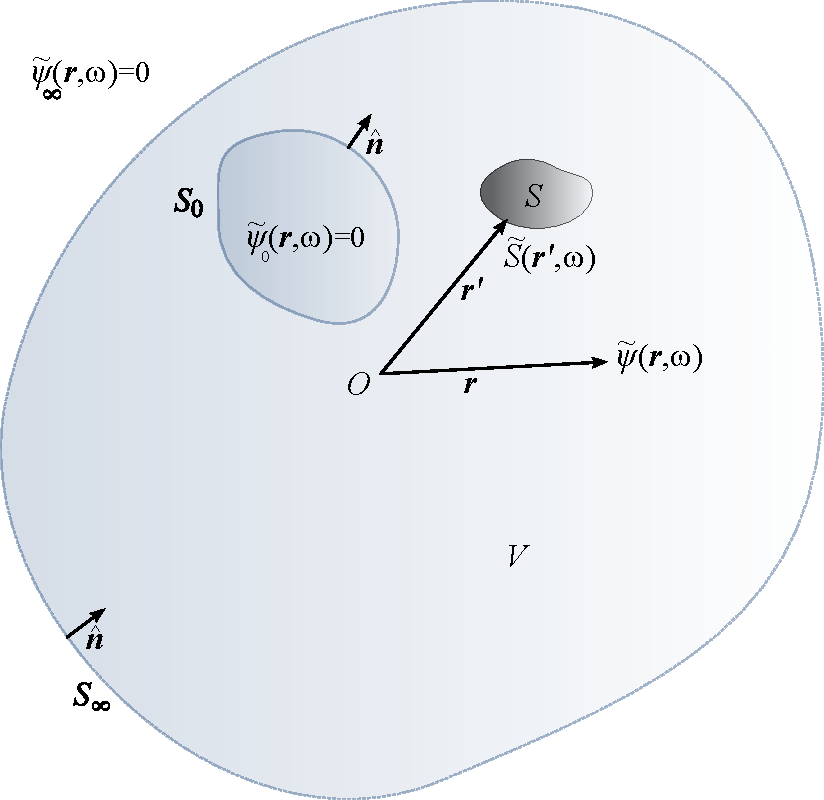
\includegraphics[width=8cm]{EMProblem} 
\caption{Electromagnetic radiation by arbitrary source distribution in an bounded medium.}
\label{fig:EMProblem}
\end{figure}
%
The figure \ref{fig:EMProblem} illustrates the geometry of the problem: a volume $V$, determined by the space between the arbitrarily shaped surfaces $\mrm{S}_0$  and $\mrm{S}_\infty$, contains an arbitrarily shaped source distribution $S$, and the vector $\mbfit{r'}$ points to the \itt{infinitesimal source element} or \itt{point source} $\tilde{S}(\mbfit{r'},\omega)$. The unit vector $\hat{\mbfit{n}}$ normal to the surfaces is chosen to be inwardly directed to $V$.
%
\par As previously said, the solution of this problem consists of solving the frequency domain Helmholtz wave equation \eqref{eq:scalHelm} where $\tilde{\psi}(\mbfit{r'}; \omega)$ is any of the components of the vector fields. To solve $\tilde{\psi}(\mbfit{r}; \omega)$ we must know the field produced by a point source, assuming that the field are given by the superposition\footnote{According to the linearity property of Maxwell's equations, in particular of the operators $\nabla \cdot$, $\nabla \times$ and $\nabla$.} of the field produced by each point source. This is the \textit{Green's function} denoted $G(\mbfit{r}|\mbfit{r'}; \omega)$ and corresponds to the field produced in $\mbfit{r}$ by a point source located in $\mbfit{r'}$ \cite{VBladelEF}
\begin{equation}
\label{eq:GreenHelmholtz}
(\nabla^2 + k^2) G(\mbfit{r}|\mbfit{r'}; \omega) = \delta (\mbfit{r} - \mbfit{r'}),
\end{equation} where $\delta$ is the Dirac delta, function of the position $\mbfit{r}$.
\par Furthermore, a solution to the Helmholtz equation \eqref{eq:scalHelm} can be obtained using the \textit{Green's second identity} \cite{RothwellCloudE} based on the following identity
\begin{equation}
\label{eq:Green2ndId}
\nabla \cdot (\Phi \nabla \Psi - \Psi \nabla \Phi) = \Phi \nabla^2 \Psi - \Psi \nabla^2 \Phi,
\end{equation} where $\Phi$ and $\Psi$ are arbitrary scalar fields, then integrating over the volume V with respect to the dummy variable $\mbfit{r'}$ and using the \itt{divergence theorem}
\begin{eqnarray}
\int_V {\nabla}' \cdot \mbfit{\Omega} \ dV'  &= & - \oint_S \mbfit{\Omega} \cdot \hat{\mbfit{n}} \ dS', \label{eq:divTh}
\end{eqnarray}
where $\mbfit{\Omega}$ is a vector-valued function of the space\footnote{Notice that the gradient of a scalar function of the space is a vector function.} and $\hat{\mbfit{n}}$ points inward to $V$. Assuming $\Phi = \tilde{\psi}(\mbfit{r'}; \omega)$ and $\Psi = G(\mbfit{r}|\mbfit{r'}; \omega)$, we obtain
\begin{eqnarray}
\label{eq:Int1}
& &\int_V \left [ \tilde{\psi}(\mbfit{r'}; \omega) {\nabla}'^2 G(\mbfit{r}|\mbfit{r'}; \omega) - G(\mbfit{r}|\mbfit{r'}; \omega) {\nabla}'^2  \tilde{\psi}(\mbfit{r'}; \omega) \right ] dV'  =  \nonumber \\ 
& &\hspace{1cm} - \oint_S \left [  \tilde{\psi}(\mbfit{r'}; \omega) {\nabla}' G(\mbfit{r}|\mbfit{r'}; \omega) - G(\mbfit{r}|\mbfit{r'}; \omega) {\nabla}' \tilde{\psi}(\mbfit{r'}; \omega) \right ] \cdot \hat{\mbfit{n}} \ dS'.
\end{eqnarray} Since $\frac{\partial{}}{\partial{n'}} = \hat{\mbfit{n}} \cdot {\nabla}'$, we can rewrite the right-hand side of \eqref{eq:Int1} in the following manner
\begin{eqnarray}
\label{eq:Int2}
& &\int_V \left [ \tilde{\psi}(\mbfit{r'}; \omega) {\nabla}'^2 G(\mbfit{r}|\mbfit{r'}; \omega) - G(\mbfit{r}|\mbfit{r'}; \omega) {\nabla}'^2  \tilde{\psi}(\mbfit{r'}; \omega) \right ] dV' =  \nonumber \\ 
& & \hspace{1cm} - \oint_{S_0+S_{\infty}} \left [ \tilde{\psi}(\mbfit{r'}; \omega) \frac{ \partial G(\mbfit{r}|\mbfit{r'}; \omega) }{\partial{n'}} - G(\mbfit{r}|\mbfit{r'}; \omega) \frac{\partial{\tilde{\psi}(\mbfit{r'}; \omega)}}{\partial{n'}} \right ]  dS'.
\end{eqnarray} Then, applying the substitutions $$\nabla^2 \tilde{\psi}(\mbfit{r'}; \omega) = - k^2 \tilde{\psi}(\mbfit{r'}; \omega) - \tilde{S}(\mbfit{r'}, \omega)$$ and $$\nabla^2 G(\mbfit{r}|\mbfit{r'}; \omega) = - k^2 G(\mbfit{r}|\mbfit{r'}; \omega) - \delta (\mbfit{r} - \mbfit{r'})$$ derived from (\ref{eq:scalHelm}-\ref{eq:GreenHelmholtz}) in the left-hand side of equation \eqref{eq:Int2}, we obtain
\begin{eqnarray}
\int_V \left [ \tilde{\psi}(\mbfit{r'}; \omega) \left ( - k^2 G(\mbfit{r}|\mbfit{r'}; \omega) - \delta (\mbfit{r} - \mbfit{r'}) \right ) - \right. \nonumber \\
& & \hspace{-7.5cm} \left. G(\mbfit{r}|\mbfit{r'}; \omega) \left (- k^2 \tilde{\psi}(\mbfit{r'}; \omega) - \tilde{S}(\mbfit{r'}; \omega) \right ) \right ] dV' =  \nonumber \\
& & \hspace{-7cm} - \oint_{S_0+S_{\infty}} \left [ \tilde{\psi}(\mbfit{r'}; \omega) \frac{ \partial G(\mbfit{r}|\mbfit{r'}; \omega) }{\partial{n'}} - G(\mbfit{r}|\mbfit{r'}; \omega) \frac{\partial{\tilde{\psi}(\mbfit{r'}; \omega)}}{\partial{n'}} \right ] dS'.
\end{eqnarray} Being equivalent, the terms with the wavenumber $k$ vanish, and the sifting property of the Dirac delta gives the following equation
\begin{eqnarray}
\label{eq:Int3}
\tilde{\psi}(\mbfit{r}; \omega) &= &\int_V G(\mbfit{r}|\mbfit{r'}; \omega) \tilde{S}(\mbfit{r'}; \omega) \ dV'  + \nonumber \\ 
& & \hspace{-1cm} \oint_{S_0+S_{\infty}} \left [  \tilde{\psi}(\mbfit{r'}; \omega) \frac{ \partial G(\mbfit{r}|\mbfit{r'}; \omega) }{\partial{n'}} - G(\mbfit{r}|\mbfit{r'}; \omega) \frac{\partial{\tilde{\psi}(\mbfit{r'}; \omega)}}{\partial{n'}} \right ] dS',
\end{eqnarray} if $\mbfit{r}$ is chosen to lie within $V$, otherwise $\tilde{\psi}(\mbfit{r}; \omega) = 0$\footnote{The sifting property of the Dirac delta is such that, for fields evaluated out of the integration domain, the integral becomes null as $\int_V f(\mbfit{r}' ) \delta (\mbfit{r} - \mbfit{r'}) \ dV' = 0, \ \ \forall \mbfit{r} \notin V$, $f(\mbfit{r})$ being a generic function of the space. \label{fn:Extinction}}.
%
\par The integral over $S_\infty$ vanishes when $\mbfit{r'} \rightarrow \infty$, as the field $\tilde{\psi}(\mbfit{r}; \omega)$ and its derivative go to zero for the \itt{Sommerfeld's radiation conditions}\footnote{These limits actually express the physically observable attenuation of the electromagnetic fields as we get away from the sources.} expressed by the following limits
\begin{eqnarray}
 \lim_{\mbfit{r} \to \infty} \tilde{\psi}(\mbfit{r}; \omega)  &= \ 0,\\
 \lim_{\mbfit{r} \to \infty} \left [ jk \tilde{\psi}(\mbfit{r}; \omega) + \frac{\partial}{\partial{r}} \tilde{\psi}(\mbfit{r}; \omega) \right ] &= \ 0.
\end{eqnarray} Removing the integral over $S_\infty$ means that we are removing the outer bounding surface of $V$, letting the radiation externally unbounded. This is necessary in order to compute the radiation pattern, which considers fields infinitely far away from the sources. Hence, the equation \eqref{eq:Int3} becomes
\begin{eqnarray}
\label{eq:Int4}
& &\tilde{\psi}(\mbfit{r}; \omega) = \int_V G(\mbfit{r}|\mbfit{r'}; \omega) S(\mbfit{r'}; \omega) dV'  + \nonumber \\
& &\hspace{1cm} \oint_{S_0} \left [ \tilde{\psi}(\mbfit{r'}; \omega) \frac{ \partial G(\mbfit{r}|\mbfit{r'}; \omega) }{\partial{n'}} - G(\mbfit{r}|\mbfit{r'}; \omega) \frac{\partial{\tilde{\psi}(\mbfit{r'}; \omega)}}{\partial{n'}} \right ] dS'.
\end{eqnarray} The equation \eqref{eq:Int4} states that the field $\tilde{\psi}(\mbfit{r}; \omega)$ within $V$ ($ V \equiv \mathbb{R}^3 / \{ V_{S_0} \}$), can be determined once one knows the source distribution $S$ within $V$ and the field and its normal derivative on $S_0$.

\par The problem of near field to far field transformation can be split into two parts. The first concerns in the determination of the near field over an arbitrary surface $S_C$ encompassing the whole sources distribution, that is computing the first integral of \eqref{eq:Int4} to obtain the field and its normal derivative on $S_C$, such that the sources can be excluded from $V$ in the second part. The second part uses the near field and derivative previously obtained to calculate the field in $V$. This is the scalar Huygen's principle, stated in the second integral of \eqref{eq:Int4}, which says that all the necessary informations about the sources enclosed is kept in the field they produce on the enclosing surface. The near-to-far transformation with scalar field will be discussed in section \ref{sec:ScalarN2F}. We first proceed with the extension of the radiation in a bounded medium to vector fields.

\subsection{Vector Huygens' principle} \label{sec:VectorHuygens} %%%%%%%% VECTOR HUYGENS

\begin{figure}[ht!]
\centering
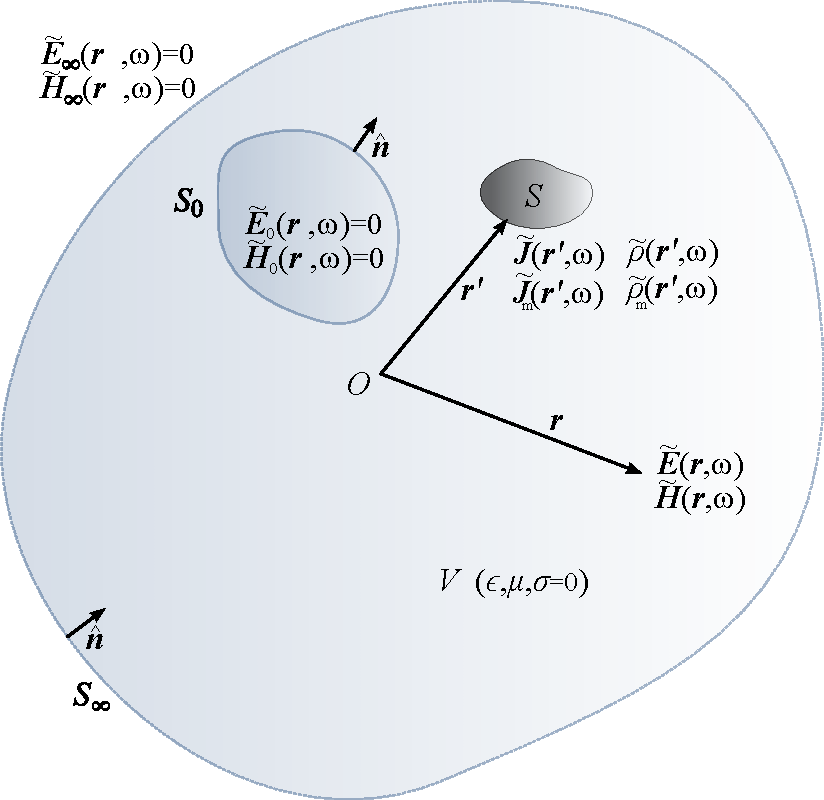
\includegraphics[width=8cm]{EMProblemVect}
\caption{Electromagnetic radiation by arbitrary currents and charges distribution in a bounded medium.}
\label{fig:EMProblemVect}
\end{figure}
\par Proceeding in the same manner as for the scalar Huygens' principle, we now use the \itt{Green's second identity} \eqref{eq:Green2ndId} extended to vector fields to compute the electric field in the bounded medium depicted in figure \ref{fig:EMProblemVect}. We obtain
\begin{eqnarray}
\label{eq:vectInt1}
\int_V \left [ \tilde{\mbfit{E}}(\mbfit{r'}; \omega) {\nabla}'^2 G(\mbfit{r}|\mbfit{r'}; \omega) - G(\mbfit{r}|\mbfit{r'}; \omega) {\nabla}'^2  \tilde{\mbfit{E}}(\mbfit{r'}; \omega) \right ] dV' &= & \nonumber \\ 
& &\hspace{-12cm} - \oint_{S_0+S_{\infty}} \left [  \tilde{\mbfit{E}}(\mbfit{r'}; \omega) \left ( \hat{\mbfit{n}} \cdot {\nabla}' G(\mbfit{r}|\mbfit{r'}; \omega) \right ) - G(\mbfit{r}|\mbfit{r'}; \omega) \left ( \hat{\mbfit{n}} \cdot {\nabla}' \tilde{\mbfit{E}}(\mbfit{r'}; \omega) \right ) \right ] \ dS',
\end{eqnarray} where $\hat{\mbfit{n}}$ is inwardly directed to $V$. We now apply to the left-hand side integrand of \eqref{eq:vectInt1} the substitutions $$ \nabla^2 \tilde{\mbfit{E}}(\mbfit{r},\omega)  = - k^2 \tilde{\mbfit{E}}(\mbfit{r},\omega) + j\omega\mu\tilde{\mbfit{J}}(\mbfit{r},\omega) + \frac{1}{\epsilon}\nabla \tilde{\rho}(\mbfit{r},\omega) + \nabla \times \tilde{\mbfit{J}}_m(\mbfit{r},\omega) $$ and $$\nabla^2 G(\mbfit{r}|\mbfit{r'}; \omega) = - k^2 G(\mbfit{r}|\mbfit{r'}; \omega) - \delta (\mbfit{r} - \mbfit{r'})$$ respectively derived from \eqref{eq:waveHelmE} and \eqref{eq:GreenHelmholtz} to obtain the equation
\begin{eqnarray}
\label{eq:vectInt2}
& &\int_V \left [ - \tilde{\mbfit{E}} \ \delta (\mbfit{r} - \mbfit{r'}) - G \left ( j\omega\mu\tilde{\mbfit{J}} + \frac{1}{\epsilon} {\nabla}' \tilde{\rho} + {\nabla}' \times \tilde{\mbfit{J}}_m \right ) \right ] dV' = \nonumber \\ 
& &\hspace{0.5cm} - \oint_{S_0+S_{\infty}} \left [  \tilde{\mbfit{E}} \left ( \hat{\mbfit{n}} \cdot {\nabla}' G \right ) - G \left ( \hat{\mbfit{n}} \cdot {\nabla}' \tilde{\mbfit{E}} \right ) \right ] \ dS',
\end{eqnarray} where, for compactness in notation, we have made the substitutions $\tilde{\mbfit{E}} = \tilde{\mbfit{E}}(\mbfit{r'}; \omega)$, $G = G(\mbfit{r}|\mbfit{r'}; \omega)$, $\tilde{\mbfit{J}} = \tilde{\mbfit{J}}(\mbfit{r'},\omega)$, $\tilde{\rho} = \tilde{\rho}(\mbfit{r'},\omega)$ and $\tilde{\mbfit{J}}_m = \tilde{\mbfit{J}}_m(\mbfit{r'},\omega)$. Once again, the terms with the wavenumber $k$ have cancelled each other. The sifting property of the Dirac delta allows the calculation of the field $\tilde{\mbfit{E}}(\mbfit{r}; \omega)$ in an arbitrary point of $V$ (elsewhere null, see note \ref{fn:Extinction}), and \eqref{eq:vectInt2} becomes
\begin{eqnarray}
\label{eq:vectInt3}
& &\tilde{\mbfit{E}}(\mbfit{r}; \omega) = - \int_V \left [ G \left ( j\omega\mu\tilde{\mbfit{J}} + \frac{1}{\epsilon} {\nabla}' \tilde{\rho} + {\nabla}' \times \tilde{\mbfit{J}}_m \right ) \right ] dV'  + \nonumber \\ 
& &\hspace{0.5cm} \oint_{S_0+S_{\infty}} \left [  \tilde{\mbfit{E}} \left ( \hat{\mbfit{n}} \cdot {\nabla}' G \right ) - G \left ( \hat{\mbfit{n}} \cdot {\nabla}' \tilde{\mbfit{E}} \right ) \right ] \ dS'.
\end{eqnarray} Using the integral theorems (respectively the \itt{gradient theorem} and the \itt{curl theorem}) \cite{RothwellCloudE}
\begin{eqnarray} %%%%%%% INTEGRALTHEOREMS
\int_V {\nabla}' \Psi \ dV' &= & - \oint_S \Psi \cdot \hat{\mbfit{n}} \ {dS'}, \\ 
\int_V {\nabla}' \times \mbfit{\Omega} \ dV' &= & - \oint_S \hat{\mbfit{n}} \times \mbfit{\Omega} \ {dS'},
\end{eqnarray} with $\hat{\mbfit{n}}$ pointing inward to $V$, one can rewrite the first integral term of right-hand side of \eqref{eq:vectInt3} as
\begin{eqnarray}
\label{eq:vectInt4} %%%%%%% 1st integral
& & - \int_V \left [ j\omega\mu G \tilde{\mbfit{J}} + \frac{1}{\epsilon} G {\nabla}' \tilde{\rho} + G {\nabla}' \times \tilde{\mbfit{J}}_m \right ] dV' = \nonumber \\
& &\hspace{0.5cm} - \int_V \left [ j\omega\mu G \tilde{\mbfit{J}} - \frac{1}{\epsilon} \tilde{\rho} {\nabla}' G + \tilde{\mbfit{J}}_m \times {\nabla}' G \right ] dV' + \nonumber \\
& &\hspace{1cm} \oint_{S_0+S_{\infty}} \left [ \hat{\mbfit{n}} \frac{1}{\epsilon} \tilde{\rho} G + \hat{\mbfit{n}} \times \tilde{\mbfit{J}}_m G \right ] \ dS',
\end{eqnarray} where the vector identities \cite{OrfanidisEWA}
\begin{eqnarray}
\nabla (\Psi \Phi) &= & \Psi \nabla \Phi + \Phi \nabla \Psi, \\
\nabla \times (\Psi \mbfit{\Omega}) &= & \Psi \nabla \times \mbfit{\Omega} + \nabla \Phi \times \mbfit{\Omega},
\end{eqnarray} have been employed with $\Psi = G$, $\Phi = \tilde{\rho}$ and $\mbfit{\Omega} = \tilde{\mbfit{J}}_m$. Then, using the following vector identity \cite{OrfanidisEWA}
\begin{eqnarray}
& &\Psi (\hat{\mbfit{n}} \cdot \nabla \mbfit{\Omega}) - \mbfit{\Omega} (\hat{\mbfit{n}} \cdot \nabla \Psi) = \left [  \hat{\mbfit{n}} \cdot \nabla \left ( \Psi \mbfit{\Omega} \right ) + \hat{\mbfit{n}} \times \left ( \nabla \times \left ( \Psi \mbfit{\Omega} \right )  \right ) - \hat{\mbfit{n}} \nabla \cdot \left ( \Psi \mbfit{\Omega} \right ) \right ] + \nonumber \\
& &\hspace{.5cm}\left [ \hat{\mbfit{n}} \Psi \nabla \cdot \mbfit{\Omega}  - \left ( \hat{\mbfit{n}} \times \mbfit{\Omega} \right ) \times \nabla \Psi - \Psi \hat{\mbfit{n}} \times \left ( \nabla \times \mbfit{\Omega} \right )  - \left ( \hat{\mbfit{n}} \cdot \mbfit{\Omega}  \right ) \nabla \Psi \right ],
\end{eqnarray} and assuming $\Psi = G$ and $\mbfit{\Omega} = \tilde{\mbfit{E}}$, the second integrand term in the right-hand side of \eqref{eq:vectInt3} can be expressed as
\begin{eqnarray}
\label{eq:vectInt5} 
& & \oint_{S_0+S_{\infty}} \left [\tilde{\mbfit{E}} \left ( \hat{\mbfit{n}} \cdot {\nabla}' G \right ) - G \left ( \hat{\mbfit{n}} \cdot {\nabla}' \tilde{\mbfit{E}} \right ) \right ] \ dS' =  \nonumber \\
& & \hspace{-0.5cm} - \oint_{S_0+S_{\infty}} \left [  \hat{\mbfit{n}} \cdot {\nabla}' \left ( G \tilde{\mbfit{E}} \right ) + \hat{\mbfit{n}} \times \left ( {\nabla}' \times \left (  G \tilde{\mbfit{E}} \right ) \right ) \hat{\mbfit{n}} {\nabla}' \cdot \left (  G \tilde{\mbfit{E}} \right ) \right ] \ dS' \ +  \nonumber \\
& & \hspace{-1cm} - \oint_{S_0+S_{\infty}} \left [ \hat{\mbfit{n}}  G {\nabla}' \cdot \tilde{\mbfit{E}} - \left ( \hat{\mbfit{n}} \times \tilde{\mbfit{E}} \right ) \times {\nabla}'  G \ - G \hat{\mbfit{n}} \times \left ( {\nabla}' \times \tilde{\mbfit{E}} \right )  - \left ( \hat{\mbfit{n}} \cdot \tilde{\mbfit{E}}  \right ) {\nabla}'  G \right ] \ dS'.
\end{eqnarray} The integral theorem \cite{OrfanidisEWA}
\begin{eqnarray}
& &\oint_S \left ( \hat{\mbfit{n}} \times {\nabla}' \right ) \times \left ( \Psi \mbfit{\Omega} \right ) \ dS \ = \ 0 \ = \nonumber \\
& &\hspace{.5cm} \oint_S \left [ \hat{\mbfit{n}} \times \left ( {\nabla}' \times\left ( \Psi \mbfit{\Omega} \right ) \right ) + \left ( \hat{\mbfit{n}} \cdot {\nabla}' \right ) \left ( \Psi \mbfit{\Omega} \right ) - \hat{\mbfit{n}} \left ( {\nabla}' \cdot \left ( \Psi \mbfit{\Omega} \right ) \right ) \right] dS
\end{eqnarray} allows us to neglect the first integral term in right-hand side of \eqref{eq:vectInt5}, and \eqref{eq:vectInt3} can be expressed as
\begin{eqnarray}
\label{eq:vectInt6} %%%%%%%% pre Stratton-Chu
& &\tilde{\mbfit{E}}(\mbfit{r}; \omega) = - \int_V \left [ j\omega\mu G \tilde{\mbfit{J}} - \frac{1}{\epsilon} \tilde{\rho} {\nabla}' G + \tilde{\mbfit{J}}_m \times {\nabla}' G \right ] dV' + \nonumber \\
& & \hspace{1cm} \oint_{S_0+S_{\infty}} \left [ \hat{\mbfit{n}} \frac{1}{\epsilon} \tilde{\rho} G + \hat{\mbfit{n}} \times \tilde{\mbfit{J}}_m G \right ] \ dS' -  \nonumber \\
& & \hspace{-1cm}\oint_{S_0+S_{\infty}} \left [ \hat{\mbfit{n}}  G {\nabla}' \cdot \tilde{\mbfit{E}}  - \left ( \hat{\mbfit{n}} \times \tilde{\mbfit{E}} \right ) \times {\nabla}'  G \ - G \hat{\mbfit{n}} \times \left ( {\nabla}' \times \tilde{\mbfit{E}} \right )  - \left ( \hat{\mbfit{n}} \cdot \tilde{\mbfit{E}}  \right ) {\nabla}' G \right ] \ dS'
\end{eqnarray} The divergence and curl of the electric field terms in the integrand of the third surface integral of right-hand side of \eqref{eq:vectInt6} can be substituted, respectively, using the Poisson's equation \eqref{eq:sfPoissonSubs} and the symmetrized Faraday's law \eqref{eq:sffaraday} together with the constitutive relation of the magnetic field \eqref{eq:ffsconst2}. As a result, the second integral of right-hand side of \eqref{eq:vectInt6} vanishes and we obtain 
\begin{eqnarray}
\label{eq:StrattonChuE}
& &\tilde{\mbfit{E}}(\mbfit{r}; \omega) =  \int_V \left [ - j\omega\mu G \tilde{\mbfit{J}} + \frac{1}{\epsilon} \tilde{\rho} {\nabla}' G - \tilde{\mbfit{J}}_m {\nabla}' \times G \right ] dV' + \nonumber \\
& & \hspace{.5cm}\oint_{S_0+S_{\infty}} \left [ - j\omega \mu G \left ( \hat{\mbfit{n}} \times \tilde{\mbfit{H}} \right ) + \left ( \hat{\mbfit{n}} \cdot \tilde{\mbfit{E}} \right ) {\nabla}'  G + \left ( \hat{\mbfit{n}} \times \tilde{\mbfit{E}} \right ) \times {\nabla}' G  \right ] \ dS',
\end{eqnarray} where $\tilde{\mbfit{H}} = \tilde{\mbfit{H}}(\mbfit{r'}; \omega)$. Then, considering the medium externally unbounded, that is letting the bounding surface $S_\infty$ going far away from the sources positions and applying the \itt{Sommerfeld's radiation conditions} for vector fields \cite{RothwellCloudE}
\begin{eqnarray}
\lim_{\mbfit{r} \to \infty} r \tilde{\mbfit{E}}(\mbfit{r}; \omega)  &< &\infty,\\
\lim_{\mbfit{r} \to \infty} r \left [ \zeta \hat{\mbfit{r}} \times \tilde{\mbfit{H}}(\mbfit{r}; \omega) +  \tilde{\mbfit{E}}(\mbfit{r}; \omega) \right ] &= &0,
\end{eqnarray} with $\zeta = \sqrt{\frac{\mu}{\epsilon}} = \zeta_0 \sqrt{\frac{\mu_r}{\epsilon_r}}$, $\zeta_0 \approx 376.73 [\Omega]$ the \itt{free-space impedance}, we obtain the following equation for the electric field
\begin{eqnarray}
\label{eq:StrattonChuUnboundedE}
& &\tilde{\mbfit{E}}(\mbfit{r}; \omega) =  \int_V \left [ - j\omega\mu G \tilde{\mbfit{J}} + \frac{1}{\epsilon} \tilde{\rho} {\nabla}' G - \tilde{\mbfit{J}}_m {\nabla}' \times G \right ] dV' + \nonumber \\
& & \hspace{.5cm}\oint_{S_0} \left [ - j\omega \mu G \left ( \hat{\mbfit{n}} \times \tilde{\mbfit{H}} \right ) + \left ( \hat{\mbfit{n}} \cdot \tilde{\mbfit{E}}  \right ) {\nabla}'  G + \left ( \hat{\mbfit{n}} \times \tilde{\mbfit{E}} \right ) \times {\nabla}' G \right ] \ dS'.
\end{eqnarray}
\par Proceeding analogously, we derive an equation for the magnetic field
\begin{eqnarray}
\label{eq:StrattonChuUnboundedH}
\tilde{\mbfit{H}}(\mbfit{r}; \omega) &= & \int_V \left [ - j\omega\epsilon G \tilde{\mbfit{J}}_m + \frac{1}{\mu} \tilde{\rho}_m {\nabla}' G - \tilde{\mbfit{J}} {\nabla}' \times G \right ] dV' + \nonumber \\
& & \hspace{-2cm}\oint_{S_0} \left [  j\omega \epsilon G \left ( \hat{\mbfit{n}} \times \tilde{\mbfit{E}} \right ) + \left ( \hat{\mbfit{n}} \cdot \tilde{\mbfit{H}}  \right ) {\nabla}' G + \left ( \hat{\mbfit{n}} \times \tilde{\mbfit{H}} \right ) \times {\nabla}' G\right ] \ dS',
\end{eqnarray} with the additional equivalence $\tilde{\rho}_m = \tilde{\rho}_m(\mbfit{r'},\omega)$. The radiation conditions corresponding to \eqref{eq:StrattonChuUnboundedH} are
\begin{eqnarray}
\lim_{\mbfit{r} \to \infty} r \tilde{\mbfit{H}}(\mbfit{r}; \omega)  &< &\infty,\\
\lim_{\mbfit{r} \to \infty} r \left [ \zeta \tilde{\mbfit{H}}(\mbfit{r}; \omega) - \hat{\mbfit{r}} \times \tilde{\mbfit{E}}(\mbfit{r}; \omega) \right ] &= & 0.
\end{eqnarray}

\par Equations \eqref{eq:StrattonChuUnboundedE} and \eqref{eq:StrattonChuUnboundedH} are the so-called \itt{Stratton-Chu formulas} \cite{StrattonET} which, similarly to \eqref{eq:Int4} for the scalar field, have two integrals: the first one dealing with the direct computation of the fields from sources distributions, the second one to formulate the vector Huygen's principle. 

\par It is to be noted that, for the fields extinction out of $V$ and for the continuity equations of the fields (\ref{eq:conte}-\ref{eq:contb})\footnote{$\tilde{\mbfit{E}}_2(\mbfit{r'}; \omega) = \tilde{\mbfit{H}}_2(\mbfit{r'}; \omega) = 0$, $\tilde{\mbfit{E}}(\mbfit{r'}; \omega) = \tilde{\mbfit{H}}_1(\mbfit{r'}; \omega)$, $\tilde{\mbfit{H}}(\mbfit{r'}; \omega) = \tilde{\mbfit{H}}_1(\mbfit{r'}; \omega)$ and $\hat{\mbfit{n}}$ inwardly directed to $V$ (region 1).}, the terms $\hat{\mbfit{n}} \times \tilde{\mbfit{E}}(\mbfit{r'}; \omega)$, $\hat{\mbfit{n}} \times \tilde{\mbfit{H}}(\mbfit{r'}; \omega)$, $\hat{\mbfit{n}} \cdot \tilde{\mbfit{E}}(\mbfit{r'}; \omega)$ and $\hat{\mbfit{n}} \cdot \tilde{\mbfit{H}}(\mbfit{r'}; \omega)$ in the second integrands of \eqref{eq:StrattonChuUnboundedE} and \eqref{eq:StrattonChuUnboundedH} correspond to, respectively, the surface currents $-\tilde\mbfit{{J}}_{ms}(\mbfit{r},\omega)$ and $\tilde{\mbfit{J}}_{s}(\mbfit{r},\omega)$, and surface charges related terms ${\epsilon}^{-1} \ \tilde{\rho}_{s}(\mbfit{r},\omega)$ and ${\mu}^{-1} \ \tilde{\rho}_{ms}(\mbfit{r},\omega)$, all of them located on $S_0$. These surface sources are also named \itt{equivalent sources} as they take place to represent the equivalent unbounded electromagnetic problem.
\par For a practical use of the Stratton-Chu formulas (\ref{eq:StrattonChuUnboundedE}-\ref{eq:StrattonChuUnboundedH}), it is interesting to convert them into a form that does not contain charge densities sources and equivalent surface charge densities. This is achieved with the use of the continuity equations for the charges \eqref{eq:contJ} and \eqref{eq:contJm}. We begin for the electric field, recasting the second integrand term of the first integral of \eqref{eq:StrattonChuUnboundedE} in the following manner:
\begin{eqnarray}
\int_V \frac{1}{\epsilon} \tilde{\rho} {\nabla}' G \ dV' &= &  - \frac{1}{j \omega \epsilon} \int_V \left ( {\nabla}' \cdot \tilde{\mbfit{J}}  \right ) {\nabla}' G \ dV' \nonumber \\
&= & - \frac{1}{j \omega \epsilon} \left [ \int_V {\nabla}' \cdot \left ( \tilde{\mbfit{J}} {\nabla}' G  \right ) dV' - \right. \nonumber \\
&  & \hspace{0.5cm} \left. \int_V \left ( \tilde{\mbfit{J}} \cdot {\nabla}' \right )  {\nabla}' G \  dV' \right ], \label{eq:charge2current}
\end{eqnarray} where the vector identity \cite{RothwellCloudE}
\begin{equation}
\nabla \cdot (\mbfit{\Omega} \ \mbfit{\Psi}) = (\nabla \cdot \mbfit{\Omega}) \mbfit{\Psi} + \mbfit{\Omega} \cdot (\nabla \mbfit{\Psi}) =  (\nabla \cdot \mbfit{\Omega}) \mbfit{\Psi} + (\mbfit{\Omega} \cdot \nabla) \mbfit{\Psi}
\end{equation} have been employed with $\mbfit{\Psi} = \nabla G$ and $\mbfit{\Omega} = \tilde{\mbfit{J}}$. The first integral in right-hand side of \eqref{eq:charge2current}, for the divergence theorem \eqref{eq:divTh}, becomes
\begin{equation}
- \frac{1}{j \omega \epsilon} \int_V {\nabla}{'} \cdot \left ( \tilde{\mbfit{J}} {\nabla}{'} G  \right ) dV' = \frac{1}{j \omega \epsilon} \oint_S  \left ( \tilde{\mbfit{J}} {\nabla}{'} G  \right ) \cdot \hat{\mbfit{n}} \ dS',
\end{equation} which vanishes if the volume $V$ surrounded by $S$ is chosen such that it slightly exceed that needed to contain the impressed sources. Thus, \eqref{eq:charge2current} becomes
\begin{eqnarray}
\int_V \frac{1}{\epsilon} \tilde{\rho} {\nabla}{'} G \ dV' &= & \frac{1}{j \omega \epsilon} \int_V \left ( \tilde{\mbfit{J}} \cdot {\nabla}{'} \right ) {\nabla}{'} G \ dV'. \label{eq:charge2currentFinal}
\end{eqnarray} Assuming now the charge and current densities of \eqref{eq:charge2currentFinal} to be located on the surface $S_0$ (to be of surface kind) and using the continuity equations (\ref{eq:conte}-\ref{eq:contb}), we can write
\begin{eqnarray}
& &\int_V \left [ j \omega \tilde{\rho}_s - \left ( \tilde{\mbfit{J}}_s \cdot {\nabla}' \right ) \right ]  {\nabla}' G \ dV' = \ \ 0 \ \ =  \nonumber \\
& & \hspace{0.5cm} \ \oint_{S_0} \left [ j \omega \epsilon \left ( \hat{\mbfit{n}} \cdot \tilde{\mbfit{E}} \right )  - \left ( \left ( \hat{\mbfit{n}} \times \tilde{\mbfit{H}} \right ) \cdot {\nabla}' \right ) \right ] {\nabla}' G \ dS'\label{eq:charge2currentSubstitutions}. 
\end{eqnarray} Thus, the Stratton-Chu equation for the electric field \eqref{eq:StrattonChuUnboundedE} can be rewritten into the following \itt{Kottler's form} \cite{OrfanidisEWA}
\begin{eqnarray}
\label{eq:KottlerE}
\tilde{\mbfit{E}}(\mbfit{r}; \omega) &= & \frac{1}{j \omega \epsilon} \int_V \left [ k^2 G \tilde{\mbfit{J}} + \left ( \tilde{\mbfit{J}} \cdot {\nabla}' \right )  {\nabla}' G - j \omega \epsilon \tilde{\mbfit{J}}_m  \times {\nabla}' G \right ] dV' + \nonumber \\
& & \hspace{-2.75cm} \frac{1}{j \omega \epsilon} \oint_{S_0} \left [  k^2 G \left ( \hat{\mbfit{n}} \times \tilde{\mbfit{H}} \right ) +  \left ( \left ( \hat{\mbfit{n}} \times \tilde{\mbfit{H}} \right ) \cdot {\nabla}' \right ) {\nabla}'  G  + j \omega \epsilon \left ( \hat{\mbfit{n}} \times \tilde{\mbfit{E}} \right ) \times {\nabla}' G \right ] \ dS'.
\end{eqnarray} Analogously for the magnetic field, \eqref{eq:StrattonChuUnboundedH} becomes
\begin{eqnarray}
\label{eq:KottlerH}
\tilde{\mbfit{H}}(\mbfit{r}; \omega) &= & \frac{1}{j \omega \mu} \int_V \left [ k^2 G \tilde{\mbfit{J}}_m + \left ( \tilde{\mbfit{J}}_m \cdot {\nabla}' \right )  {\nabla}' G + j \omega \mu \tilde{\mbfit{J}}  \times {\nabla}' G \right ] dV' + \nonumber \\
& & \hspace{-2.75cm} \frac{1}{j \omega \mu} \oint_{S_0} \left [ - k^2 G \left ( \hat{\mbfit{n}} \times \tilde{\mbfit{E}} \right ) - \left ( \left ( \hat{\mbfit{n}} \times \tilde{\mbfit{E}} \right ) \cdot {\nabla}' \right ) {\nabla}' G + j \omega \mu \left ( \hat{\mbfit{n}} \times \tilde{\mbfit{H}} \right ) \times {\nabla}' G \right ] \ dS'.
\end{eqnarray} The surface integrals of Kottler's equations (\ref{eq:KottlerE}-\ref{eq:KottlerH}) state the so-called \itt{Love's equivalence principle } \cite{RothwellCloudE} while considering the \itt{equivalent electric and magnetic currents} $\tilde{\mbfit{J}}_s^{eq} =  \hat{\mbfit{n}} \times \tilde{\mbfit{H}}$ and $\tilde{\mbfit{J}}_{ms}^{eq} = - \hat{\mbfit{n}} \times \tilde{\mbfit{E}}$ on the bounding surface $S_0$.

%%%%%%%%%%%%%%%%%%%%%%%%%%%%%%%%%%%%%%%%%%%%%%%%%%%%%%%%%%%%%%%%%%%%%%%%%%%%%%%%%%%%%%%%%%%%%%%%%%%%%%%%%%%%%%%%%%%%%%%%%%%%%%%%%%%%%%%%%%%
%%%%%%%%%%%%%%%%%%%%%%%%%%%%%%%%%%%%%%%%%%%%%%%%%% N2F scalar
\section{Scalar near field to far field transformation} \label{sec:ScalarN2F}

\par In this section, we present a numerical implementation of the scalar near field to far field transformation (scalar N2F), relying on the mathematical formulation discussed in section \ref{sec:ScalarHuygens}. We first recall in a generic form the steps to be followed for the scalar N2F, then a computation will be performed in Matlab\footnote{Matlab${}^{\copyright}$ Mathworks. Further informations available on \url{www.mathworks.com}.} environment considering as enclosing surface first a sphere then a parallelepiped. The results will be compared to the direct computation of the far fields, assuming an unbounded medium.
%
\subsection{Computation steps} \label{sec:CompSteps}
\par For the computation of the near field or \itt{Fresnel-zone } field, we need to consider the sources distributed within the volume $V_{S_C} \subset V$, determined by the arbitrary surface $S_C$, chosen to be relatively close\footnote{The distance $\frac{2 \ \mrm{L}^2}{\lambda}$, where L is the highest length in a planar distribution of point sources and $\lambda$ the wavelength,  is the distance from the sources where we commit a maximum phase error of $\nicefrac{\pi}{8}$ in the plane wave approximation directed perpendicularly to the point sources distribution. This distance can be taken as a reference for the near-zone to far-zone fields transition and the near fields are typically considered to lie within $d \ll \frac{2 \ \mrm{L}^2}{\lambda}$.\label{fn:NF2FFdist}} to the sources. We also consider the surface $S_0$ going to zero, such that the second integral term in the right-hand side of equation \eqref{eq:Int4} vanishes. We obtain:
\begin{equation}
\label{eq:IntNF}
\tilde{\psi}(\mbfit{r}; \omega) \ \Big\vert_{S_C} = \int_{V_{S_C}} G(\mbfit{r}|\mbfit{r'}; \omega) \ \tilde{S}(\mbfit{r'}, \omega) dV'
\end{equation} where $\mbfit{r'}$ is a vector pointing to an infinitesimal source element. The problem's geometry is depicted in figure \ref{fig:EMNF}. The Green's function that will be used is the well-known \itt{Green's function for free space}
\begin{equation}
\label{eq:GrFunc}
G(\mbfit{r}|\mbfit{r'}; \omega) =\frac{\mrm{e}^{-jk|\mbfit{r}-\mbfit{r'}|}}{4\pi|\mbfit{r}-\mbfit{r'}|}
\end{equation} with $k=k_0=\nicefrac{\omega}{c_0}$ and the sources will be assumed to be radiating isotropically a unit of power density, that is $\displaystyle \sum_{n=1}^N \left | \frac{ \tilde{S}_n(\mbfit{r'}, \omega)}{4 \pi} \right |^{2} = 1$, with $N$ the number of sources.
\begin{figure}[ht!]
\centering
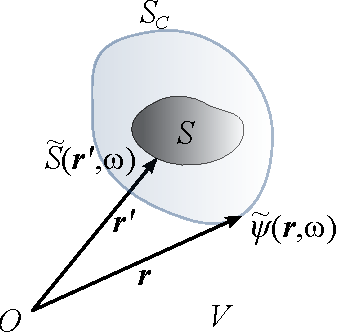
\includegraphics[width=5cm]{EMNF}
\caption{Near field computations.}
\label{fig:EMNF}
\end{figure}

\par The computation of the far field or \itt{Fraunhofer-zone} field can be performed by simply setting the modulus of the vectors $\mbfit{r}$ of a consistent number of wavelengths (see note \ref{fn:NF2FFdist}). This is the direct computation of the far field from an arbitrary sources distribution. However, we are interested in the computation of the far field not directly from the sources but from the near field they produce. Looking at equation \eqref{eq:Int4}, we see that we can achieve this by letting $S_0$ be wide enough to encompass all the sources, such that they are not anymore part of $V$ and the first integral term in the right-hand side of \eqref{eq:Int4} goes to zero. Then, from the field $\tilde{\psi}(\mbfit{r'}; \omega)$ computed over $S_0$, we compute the second integral term to obtain the field $\tilde{\psi}(\mbfit{r}; \omega) \ \forall \mbfit{r} \in V$. To make sure that the field previously calculated with \eqref{eq:IntNF} equals $\tilde{\psi}(\mbfit{r'}; \omega)$, we choose $S_0$ equal to $S_C$. Now, the expression to evaluate is
\begin{equation}
\label{eq:IntNF2FF}
\tilde{\psi}(\mbfit{r}; \omega) = \oint_{S_0 = S_C} \left [ \tilde{\psi}(\mbfit{r'}; \omega) \frac{ \partial G(\mbfit{r}|\mbfit{r'}; \omega) }{\partial{n'}} - G(\mbfit{r}|\mbfit{r'}; \omega) \frac{\partial{\tilde{\psi}(\mbfit{r'}; \omega)}}{\partial{n'}} \right ] dS'.
\end{equation} The scalar N2F step is depicted in figure \ref{fig:EMNF2FF}.
\begin{figure}[ht!]
\centering
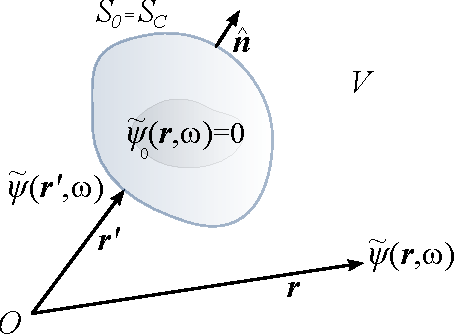
\includegraphics[width=5cm]{EMNF2FF}
\caption{Near field to far field transformation.}
\label{fig:EMNF2FF}
\end{figure}
%%%%%%%%%%%%%%%%%%%%%%%%%%%%%%%%%%%%%%%%%%%%%%%%%%%%%%%%%% NF2FF from Sphere
\subsection{Computations on a bounding sphere}

\par Let us now assume the bounding surface $S_0 = S_C$ to be a sphere, and the origin of the reference system $O$ to be located at the center of the sphere. The geometry of the problem is depicted in figure \ref{fig:SphereNF2FF}.
\begin{figure}[ht!]
\centering
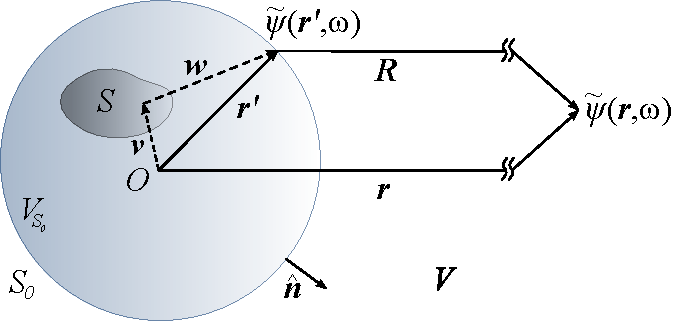
\includegraphics[width=10cm]{SphereNF2FF}
\caption{Near field to far field transformation from a bounding sphere.}
\label{fig:SphereNF2FF}
\end{figure}
The volume $V$ is the entire free space, excluded $V_{S_0}$ which contains all the sources. The spherical geometry of the problem allows us to use spherical coordinates while computing the previous relations \eqref{eq:IntNF} and \eqref{eq:IntNF2FF}.

\par The near field is computed using the \eqref{eq:IntNF} for the given geometry and we have
\begin{equation}
\label{eq:SphereIntNF}
\tilde{\psi}(\mbfit{r'}; \omega) \ \Big\vert_{S_0} = \int_{V_{S_0}} \frac{\mrm{e}^{-jk|\mbfit{r'}-\mbfit{v}|}}{4\pi|\mbfit{r'}-\mbfit{v}|} \ \tilde{S}(\mbfit{v}, \omega) d{V}_\mbfit{v}.
\end{equation} \eqref{eq:SphereIntNF} gives the value of the near field surface density on a single infinitesimal point of the sphere indicated by $\mbfit{r'}$ (i.e. determined by the Green's function) and produced by the enclosed sources distribution. 

\par We now proceed with the scalar N2F, provided that $\tilde{\psi}(\mbfit{r'}; \omega)$ and its gradient ${\nabla}' \tilde{\psi}(\mbfit{r'}; \omega)$ are known on the entire sphere.

\par Using $\frac{\mrm{e}^{-jk|\mbfit{R}|}}{4\pi|\mbfit{R}|} = \frac{\mrm{e}^{-jk|\mbfit{r}-\mbfit{r'}|}}{4\pi|\mbfit{r}-\mbfit{r'}|}$ as Green's function, the far field becomes the following
\begin{equation}
\label{eq:SphereIntNF2FF}
\tilde{\psi}(\mbfit{r}; \omega) = \oint_{S_0} \left [  \tilde{\psi}(\mbfit{r'}; \omega) \frac{ \partial{}} {\partial{n'}} \frac{\mrm{e}^{-jk|\mbfit{R}|}}{4\pi|\mbfit{R}|}  -  \frac{\mrm{e}^{-jk|\mbfit{R}|}}{4\pi|\mbfit{R}|} \frac{\partial{\tilde{\psi}(\mbfit{r'}; \omega)}}{\partial{n'}} \right ] dS'.
\end{equation} The gradient of the Green's function is
\begin{equation}
\nabla_{\mbfit{R}} \frac{\mrm{e}^{-jk|\mbfit{R}|}}{4\pi|\mbfit{R}|} = - \left ( jk + \frac{1}{|\mbfit{R}|} \right ) \frac{\mrm{e}^{-jk|\mbfit{R}|}}{4\pi|\mbfit{R}|} \frac{\mbfit{R}}{|\mbfit{R}|}
\end{equation} and its normal derivative
\begin{eqnarray}
\frac{ \partial{}} {\partial{n'}} \frac{\mrm{e}^{-jk|\mbfit{R}|}}{4\pi|\mbfit{R}|} &= & \hat{\mbfit{n}} \cdot {\nabla}' \frac{\mrm{e}^{-jk|\mbfit{r}-\mbfit{r'}|}}{4\pi|\mbfit{r}-\mbfit{r'}|} \ \ = \ \ - \hat{\mbfit{n}} \cdot {\nabla} \frac{\mrm{e}^{-jk|\mbfit{r}-\mbfit{r'}|}}{4\pi|\mbfit{r}-\mbfit{r'}|} \ \ = \ \ - \hat{\mbfit{n}} \cdot \nabla_{\mbfit{R}} \frac{\mrm{e}^{-jk|\mbfit{R}|}}{4\pi|\mbfit{R}|} \nonumber \\
&= &  \left ( jk + \frac{1}{|\mbfit{R}|} \right )  \frac{\mrm{e}^{-jk|\mbfit{R}|}}{4\pi|\mbfit{R}|} \left ( \frac{\mbfit{R}}{|\mbfit{R}|} \cdot \hat{\mbfit{n}} \right ).
\end{eqnarray} For the spherical shape of the surface $S_0$, its normal inwardly directed to $V$ is $\hat{\mbfit{n}} = \frac{\mbfit{r'}}{|\mbfit{r'}|} $ and the integral relation \eqref{eq:SphereIntNF2FF} can be rewritten as follows
\begin{eqnarray}
\label{eq:SphereIntNF2FF2}
\tilde{\psi}(\mbfit{r}; \omega) &= & \oint_{S_0} \left [  \tilde{\psi}(\mbfit{r'}; \omega) \ \left ( jk + \frac{1}{|\mbfit{R}|} \right )  \frac{\mrm{e}^{-jk|\mbfit{R}|}}{4\pi|\mbfit{R}|} \left ( \frac{\mbfit{R}}{|\mbfit{R}|} \cdot \frac{\mbfit{r'}}{|\mbfit{r'}|}  \right )  -  \frac{\mrm{e}^{-jk|\mbfit{R}|}}{4\pi|\mbfit{R}|} \frac{\partial{\tilde{\psi}(\mbfit{r'}; \omega)}}{\partial{n'}} \right ] dS' \nonumber \\
&= & \oint_{S_0} \frac{\mrm{e}^{-jk|\mbfit{R}|}}{4\pi|\mbfit{R}|} \left [ \left ( jk + \frac{1}{|\mbfit{R}|} \right )  \tilde{\psi}(\mbfit{r'}; \omega)  \left ( \frac{\mbfit{R}}{|\mbfit{R}|} \cdot \frac{\mbfit{r'}}{|\mbfit{r'}|} \right )  -  \frac{\partial{\tilde{\psi}(\mbfit{r'}; \omega)}}{\partial{n'}} \right ]  dS' \nonumber \\
&= & \oint_{S_0} \frac{\mrm{e}^{-jk|\mbfit{R}|}}{4\pi|\mbfit{R}|} \left [ \left ( jk + \frac{1}{|\mbfit{R}|} \right ) \tilde{\psi}(\mbfit{r'}; \omega)  \left ( \frac{\mbfit{R}}{|\mbfit{R}|} \cdot \frac{\mbfit{r'}}{|\mbfit{r'}|} \right )  - \right. \nonumber \\
& &  \hspace{1cm} \left. \frac{\partial{\tilde{\psi}(\mbfit{r'}; \omega)}}{\partial{r'}} \left ( \frac{\mbfit{r'}}{|\mbfit{r'}|} \cdot \frac{\mbfit{r'}}{|\mbfit{r'}|} \right ) \right ] dS' \nonumber \\
&= & \oint_{S_0} \frac{\mrm{e}^{-jk|\mbfit{R}|}}{4\pi|\mbfit{R}|}  \left [ \left ( jk + \frac{1}{|\mbfit{R}|} \right ) \tilde{\psi}(\mbfit{r'}; \omega)  \left ( \frac{\mbfit{R}}{|\mbfit{R}|} \cdot \frac{\mbfit{r'}}{|\mbfit{r'}|} \right )  - \frac{\partial{\tilde{\psi}(\mbfit{r'}; \omega)}}{\partial{r'}} \right ] dS'.
\end{eqnarray}  where we have used the identity $\frac{\partial}{\partial{n'}} =  \left ( \frac{\mbfit{r'}}{|\mbfit{r'}|} \cdot \hat{\mbfit{n}} \right ) \frac{\partial}{\partial{r'}}$.

%% approx
\par As we are only interested in the far field, we can make the following approximations for $|\mbfit{R}|$ noting that
\begin{equation}
R = \sqrt{(\mbfit{r}-\mbfit{r'}) \cdot (\mbfit{r}-\mbfit{r'}) } = \sqrt{r^2  - 2 (\mbfit{r} \cdot \mbfit{r'}) + {r'}^2},
\end{equation} such that for $\mbfit{R}$ in the far-zone we have $r \gg r'$, hence $\frac{\mbfit{R}}{|\mbfit{R}|} = \hat{\mbfit{R}} \approx \hat{\mbfit{r}}$ and the dominant terms of a Taylor expansion for the square root gives
\begin{equation}
R = r \sqrt{1 - 2 \frac{(\hat{\mbfit{r}} \cdot \mbfit{r'})}{r} + {\left (\frac{r'}{r} \right )}^2} \approx r \left [ 1 - \frac{(\hat{\mbfit{r}} \cdot \mbfit{r'})}{r} \right ] = r - \hat{\mbfit{r}} \cdot \mbfit{r'}.
\end{equation} Thus, the Green's function may be approximated as
\begin{equation}
\label{eq:GrAppr}
G(\mbfit{r}|\mbfit{r'};\omega) = \frac{\mrm{e}^{-jk|\mbfit{R}|}}{4\pi|\mbfit{R}|} \approx \frac{\mrm{e}^{-jk r}}{4\pi r} \mrm{e}^{jk \hat{\mbfit{r}} \cdot \mbfit{r'}}.
\end{equation} The integral of \eqref{eq:SphereIntNF2FF2} becomes
\begin{eqnarray}
\label{eq:SphereIntNF2FF3}
\tilde{\psi}(\mbfit{r}; \omega) \Big{|}_{r \gg r'} &\approx & \oint_{S_0} \frac{\mrm{e}^{-jk r}}{4\pi r} \mrm{e}^{jk \hat{\mbfit{r}} \cdot \mbfit{r'}}  \left [ \left ( jk + \frac{1}{r} \right ) \tilde{\psi}(\mbfit{r'}; \omega)  \left (\hat{\mbfit{r}} \cdot \hat{\mbfit{r}}' \right ) - \frac{\partial{\tilde{\psi}(\mbfit{r'}; \omega)}}{\partial{r'}} \right ] dS' \nonumber \\
&\approx & \frac{\mrm{e}^{-jk r}}{4\pi r} \oint_{S_0}  \mrm{e}^{jk \hat{\mbfit{r}} \cdot \mbfit{r'}}  \left [ \left ( jk + \frac{1}{r} \right ) \tilde{\psi}(\mbfit{r'}; \omega)  \left ( \hat{\mbfit{r}} \cdot \hat{\mbfit{r}}'  \right )  -  \frac{\partial{\tilde{\psi}(\mbfit{r'}; \omega)}}{\partial{r'}} \right ] dS' \nonumber \\
& \begin{array}[t]{c}  \approx \\[-10pt] \scriptstyle {kr \gg 1} \end{array} & \frac{\mrm{e}^{-jk r}}{4\pi r} \oint_{S_0}  \mrm{e}^{jk \hat{\mbfit{r}} \cdot \mbfit{r'}}  \left [  jk  \tilde{\psi}(\mbfit{r'}; \omega)  \left ( \hat{\mbfit{r}} \cdot \hat{\mbfit{r}}'  \right )  -  \frac{\partial{\tilde{\psi}(\mbfit{r'}; \omega)}}{\partial{r'}} \right ] dS'.
\end{eqnarray}

\par Finally, the radiation pattern is computed from \eqref{eq:SphereIntNF2FF3}, removing the distance $r$ dependence by the following limit
\begin{eqnarray}
\label{eq:SphereIntNF2FFPattern}
\mathcal{P} \left (\hat{\mbfit{r}}; \omega \right ) & = &\lim_{r \to \infty}{r^2 {\left | \tilde{\psi}(\mbfit{r}; \omega) \right |}^2 } \nonumber \\
& = & { \left | \oint_{S_0} \frac{\mrm{e}^{jk \hat{\mbfit{r}} \cdot \mbfit{r'}}}{4 \pi}  \left [ jk \tilde{\psi}(\mbfit{r'}; \omega)  \left ( \hat{\mbfit{r}} \cdot \hat{\mbfit{r}}' \right )  -  \frac{\partial{\tilde{\psi}(\mbfit{r'}; \omega)}}{\partial{r'}} \right ] dS' \right | }^2 \nonumber \\
& = & {\left |  \tilde{\psi}_r^* \right |}^2,
\end{eqnarray} where $ \tilde{\psi}_r^* \in \mathbb{C}$ is the \itt{far field detector}.

\subsubsection{Pattern in spherical coordinates}

\par For the spherical symmetry of the sphere's N2F problem, it is interesting to express the vectors $\mbfit{r}$ and $\mbfit{r'}$ with spherical variables for the computation of \eqref{eq:SphereIntNF2FFPattern}. To evaluate the scalar products, we can rely on Cartesian unit vectors basis with the components of the vectors dependent on spherical variables. The unit vectors involved in the far field detector are,
\begin{eqnarray}
\hat{\mbfit{r}}'  &=  &\cos(\theta_{r'}) \cos(\phi_{r'}) \, \hat{\mbfit{i}}_x + \cos(\theta_{r'}) \sin(\phi_{r'}) \, \hat{\mbfit{i}}_y + \sin(\theta_{r'}) \, \hat{\mbfit{i}}_z, \nonumber \\
\hat{\mbfit{r}}   &=   &\cos(\theta_{r}) \cos(\phi_{r}) \, \hat{\mbfit{i}}_x + \cos(\theta_{r}) \sin(\phi_{r}) \, \hat{\mbfit{i}}_y + \sin(\theta_{r}) \, \hat{\mbfit{i}}_z,
\end{eqnarray} and their scalar product is given by
\begin{eqnarray}
\xi(\theta_{r}, \phi_{r}, \theta_{r'}, \phi_{r'}) &= &\cos(\theta_{r}) \cos(\phi_{r}) \, \cos(\theta_{r'}) \cos(\phi_{r'}) + \nonumber \\
& & \cos(\theta_{r}) \sin(\phi_{r}) \, \cos(\theta_{r'}) \sin(\phi_{r'}) + \nonumber \\
& & \sin(\theta_{r}) \, \sin(\theta_{r'}) \nonumber \\
&= & \sin(\theta_{r}) \sin(\theta_{r'}) \cos(\phi_{r} - \phi_{r'}) + \nonumber \\ 
& & \cos(\theta_{r}) \cos(\theta_{r'}).
\end{eqnarray} The relation \eqref{eq:SphereIntNF2FFPattern} can be written as follows
\begin{eqnarray}
\label{eq:SphereIntNF2FFPatternSphCoord}
\mathcal{P} \left ( \theta_{r}, \phi_{r} ; \omega \right ) = { \left |\int_0^{2\pi}  \int_0^{\pi} \frac{\mrm{e}^{jk \, r' \, {\xi}' }}{4\pi}  \left [ jk {\tilde{\psi}_{r'}}' \, {\xi}'   -  \frac{\partial{{\tilde{\psi}_{r'}}'}}{\partial{r'}} \right ] {r'}^2 \sin({\theta_{r'}}') d{\theta_{r'}}' d{\phi_{r'}}'  \right | }^2,
\end{eqnarray} where ${\tilde{\psi}_{r'}}' = \tilde{\psi}(r', {\theta_{r'}}', {\phi_{r'}}' ; \omega)$ and ${\xi}' = \xi(\theta_{r}, \phi_{r}, {\theta_{r'}}', {\phi_{r'}}')$.

\subsubsection{Numerical implementation} \label{sec:NumImp}

\par We present the results obtained from a Matlab implementation that computes the pattern from planar array of 3 by 5 point sources ($N = 15$ point sources), the firsts disposed along the $x$ direction and the latter along $y$. The point sources or array elements are chosen to be equally spaced of $\nicefrac{\lambda}{2}$. Due to power normalization, the maximum gain the array can achieve, which is actually the \itt{directivity} as the point sources are located in a lossless medium, is given by the total number of point sources, that is $10 \ \log_{10}(N) \approx 11.76 \ \mrm{dB}$ \cite{SelleriETA}. 

\par From \eqref{eq:SphereIntNF2FF3}, we can see that the values we have to compute in the first step are the near field $ \tilde{\psi}(\mbfit{r'}; \omega) $ and its radial derivative $\frac{\partial{\tilde{\psi}(\mbfit{r'}; \omega)}}{\partial{r'}}$. The first is achieved by the numerical integration of the volume integral \eqref{eq:SphereIntNF}, considering $\tilde{S}(\mbfit{v}_n, \omega) = \tilde{S}_n \delta(\mbfit{v} - \mbfit{v}_n), n=1 \ldots N$. We obtain
\begin{eqnarray}
\label{eq:sphNumPsi}
\tilde{\psi}_m(\mbfit{r'}_m; \omega) & = & \sum_{n=1}^N \frac{\mrm{e}^{-jk|\mbfit{r'}_m-\mbfit{v}_n|}}{4\pi|\mbfit{r'}_m-\mbfit{v}_n|} \ \tilde{S}_n \qquad n=1 \ldots N, \ m=1 \ldots M
\end{eqnarray}
where we have discretized the sphere in $M$ sampling points. The second one, noting that $\tilde{S}(\mbfit{v}, \omega)$ has no dependence on the vector $\mbfit{r'}$, can be evaluated proceeding in the following manner
\begin{eqnarray}
\frac{\partial{\tilde{\psi}(\mbfit{r'}; \omega)}}{\partial{r'}} &= & \frac{\partial{}}{\partial{r'}} \int_{V_{S_0}} \frac{\mrm{e}^{-jk|\mbfit{r'}-\mbfit{v}|}}{4\pi|\mbfit{r'}-\mbfit{v}|} \ \tilde{S}(\mbfit{v}, \omega) d{V}_\mbfit{v} \nonumber \\
& = & \int_{V_{S_0}} \frac{\partial{}}{\partial{r'}} \frac{\mrm{e}^{-jk|\mbfit{r'}-\mbfit{v}|}}{4\pi|\mbfit{r'}-\mbfit{v}|} \ \tilde{S}(\mbfit{v}, \omega) d{V}_\mbfit{v} \qquad \forall \mbfit{r'} \neq \mbfit{v} \nonumber \\
& = & - \int_{V_{S_0}} \left ( jk + \frac{1}{|\mbfit{r'}-\mbfit{v}|} \right )  \frac{\mrm{e}^{-jk|\mbfit{r'}-\mbfit{v}|}}{4\pi|\mbfit{r'}-\mbfit{v}|} \left ( \frac{\mbfit{r'}-\mbfit{v}}{|\mbfit{r'}-\mbfit{v}|} \cdot \hat{\mbfit{r}}' \right ) \ \tilde{S}(\mbfit{v}, \omega) d{V}_\mbfit{v}, \qquad
\end{eqnarray} which becomes, in a numerical form,
\begin{eqnarray}
\frac{\partial{\tilde{\psi}_m(\mbfit{r'}_m; \omega)}}{\partial{r'}_m} & = & - \sum_{n=1}^N \left ( jk + \frac{1}{|\mbfit{r'}_m-\mbfit{v}_n|} \right )  \frac{\mrm{e}^{-jk|\mbfit{r'}_m-\mbfit{v}_n|}}{4\pi|\mbfit{r'}_m-\mbfit{v}_n|} \left ( \frac{\mbfit{r'}_m-\mbfit{v}_n}{|\mbfit{r'}_m-\mbfit{v}_n|} \cdot \hat{\mbfit{r}}'_m \right ) \ \tilde{S}_n \nonumber \\
& & \qquad n=1 \ldots N, \ m=1 \ldots M.
\end{eqnarray}

\par The scalar N2F from a bounding sphere, varying the sampling resolution in terms of wavelengths and using a \itt{midpoint\footnote{The fields sampling points are located in the middle of surface patches $\Delta S_n$, and an integration of a discretized function $\Phi_n$ is obtained by the sum $\sum_{n=1}^N \Phi_n \Delta S_n$. The \itt{Trapezoidal rule} have also been tested, with no significant improvement in the pattern error. Further enhancements can be achieved with \itt{Gaussian quadrature}. \cite{BondesonRylanderIngelstroemCE} \label{fn:midPointInt}} numerical integration} of \eqref{eq:SphereIntNF2FFPattern} over the sphere, will be compared to the direct computation of the pattern (the gain for several look angles). We obtain the N2F numerical formula
\begin{eqnarray}
\label{eq:sphNumPsiN2F}
\mathcal{P}_{p \mrm{N2F}} \left (\hat{\mbfit{r}}_p ; \omega \right ) & = &{\left |  \tilde{\psi}_{r_p}^* \right |}^2 \ =  \nonumber \\
& & \hspace{-4cm} { \left | \sum_{m=1}^M  \frac{\mrm{e}^{jk \hat{\mbfit{r}}_p \cdot \mbfit{r'}_m}}{4\pi}  \left [ jk \tilde{\psi}_m(\mbfit{r'}_m; \omega)  \left ( \hat{\mbfit{r}}_p \cdot \hat{\mbfit{r}}'_m \right )  -  \frac{\partial{\tilde{\psi}_m(\mbfit{r'}_m; \omega)}}{\partial{r'}_m} \right ] \Delta S_m \right | }^2. \nonumber \\
& & \qquad m=1 \ldots M, \  p=1 \ldots P.
\end{eqnarray}
The direct field computation is derived from formula \eqref{eq:sphNumPsi}, with $\mbfit{r'}_m$ to become the far-zone unit vectors $\hat{\mbfit{r}}_p$, assuming the far field approximation \eqref{eq:GrAppr} and applying the far-zone limit used in \eqref{eq:SphereIntNF2FFPattern}, that is
\begin{eqnarray}
\label{eq:sphNumPsiFar}
\mathcal{P}_{p \mrm{Direct}} \left (\hat{\mbfit{r}}_p ; \omega \right ) & = & \lim_{r_p\to\infty} r_p^2 \left | \frac{\mrm{e}^{-jk r_p}}{4\pi r_p} \sum_{n=1}^N  \mrm{e}^{jk \hat{\mbfit{r}}_p \cdot \mbfit{v}_n}  \ \tilde{S}_n \right |^2 \nonumber \\
& = & \left | \sum_{n=1}^N \frac{\mrm{e}^{jk \hat{\mbfit{r}}_p \cdot \mbfit{v}_n}}{4\pi}  \ \tilde{S}_n \right |^2 \qquad n=1 \ldots N, \  p=1 \ldots P.
\end{eqnarray}
\par The geometry of the discretized domain is depicted in figure \ref{fig:sph3x5}. The radius of the sphere is set to be radially $\nicefrac{\lambda}{2}$ away from the corner elements, i.e. $|\mbfit{r'}_m| = 1.618 \lambda$ and the angles $\theta_{r'}$ and $\phi_{r'}$ of near field sampling are computed assuming $|\mbfit{r'}_m| \Delta\theta_{r'} \approx |\mbfit{r'}_m| \Delta\phi_{r'} \approx \nicefrac{\lambda}{10}$.
\begin{figure}[ht!]
\centering
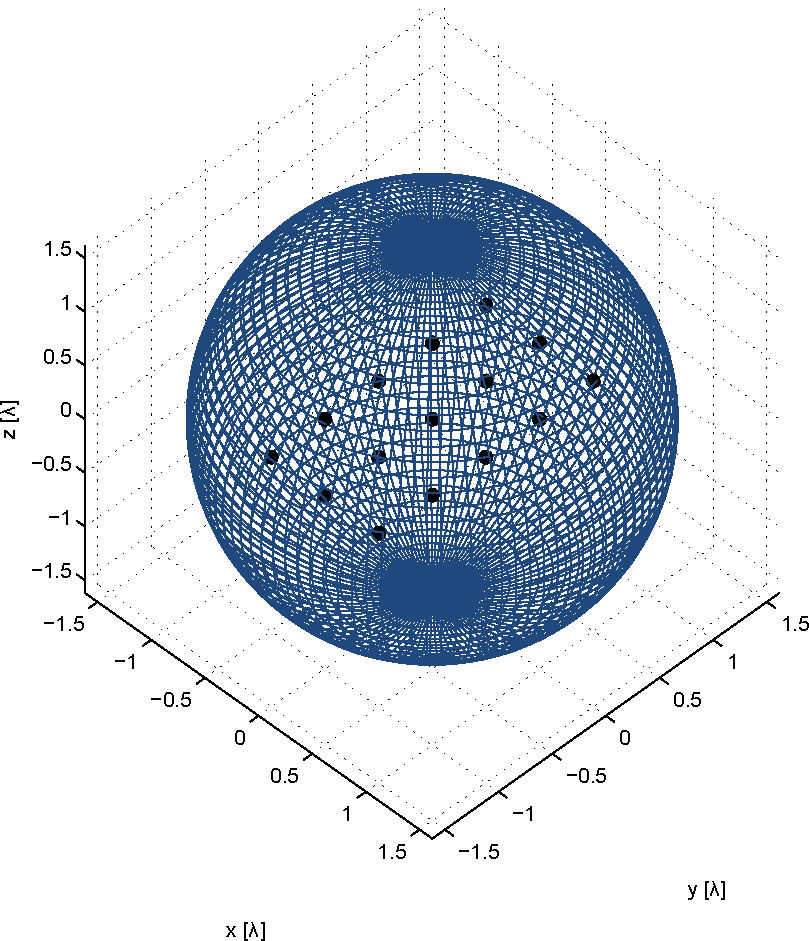
\includegraphics[width=12cm]{sph3x5}
\caption{N2F bounding sphere and 3 by 5 point sources, with $\nicefrac{\lambda}{10}$ sampling resolution.}
\label{fig:sph3x5}
\end{figure} 

\begin{figure}[!tbp]
\centering
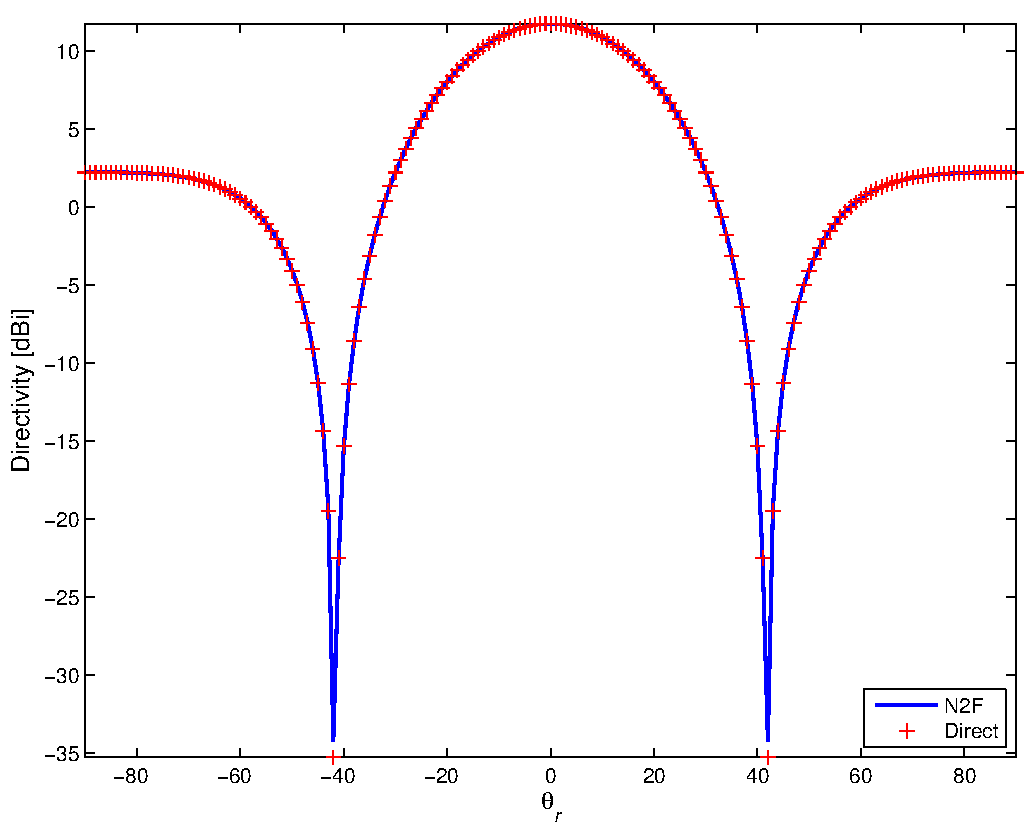
\includegraphics[width=12cm]{sph3x5_Phi0_0_0}
\caption{Pattern computed for equally phased point sources (broadside pattern) on the $\phi=0$\textdegree \ cut plane with $\nicefrac{\lambda}{10}$ sampling resolution.}
\label{fig:sph3x5_Phi0_0_0}
\end{figure}
\begin{figure}[!bp]
\centering
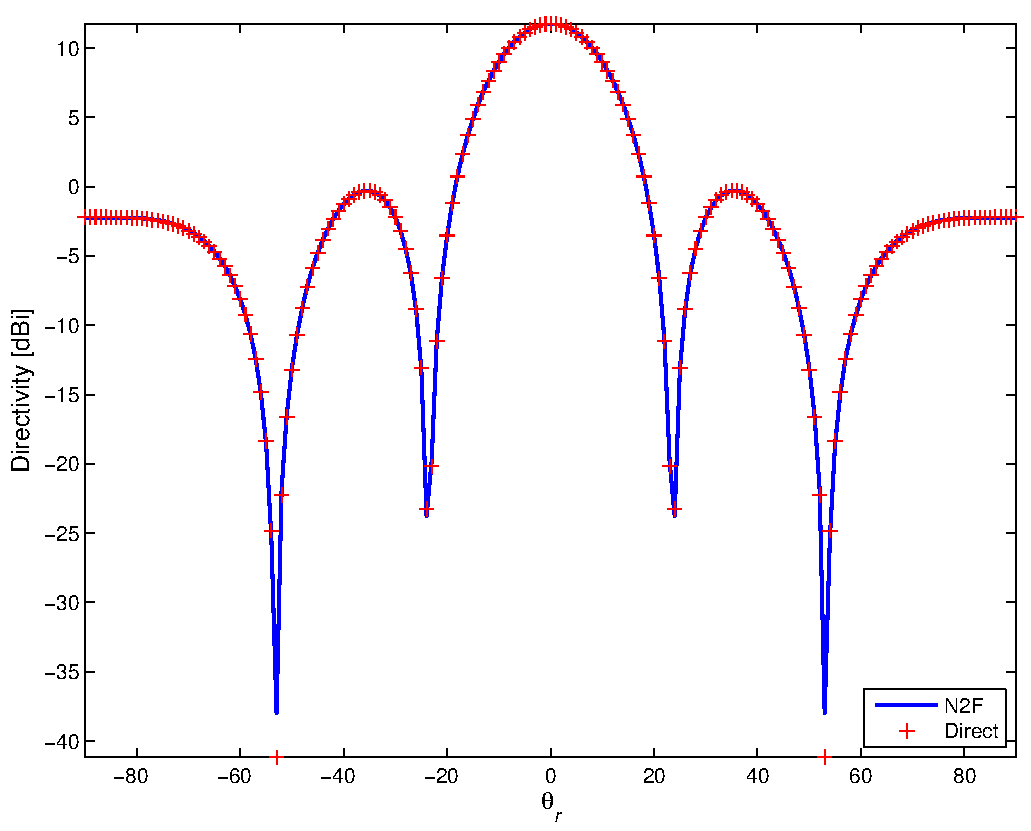
\includegraphics[width=12cm]{sph3x5_Phi90_0_0}
\caption{Pattern computed for equally phased point sources on the $\phi=90$\textdegree \ cut plane with $\nicefrac{\lambda}{10}$ sampling resolution.}
\label{fig:sph3x5_Phi90_0_0}
\end{figure}

Notice that the radial extension of the sphere from the array cannot be lower than the sampling resolution (inferior limit), and the superior limit is associated to the increasing memory consumption, in order to keep the desired resolution, as the sphere radius grows.

\par Figures \ref{fig:sph3x5_Phi0_0_0} and \ref{fig:sph3x5_Phi90_0_0} show the radiation patterns computed\footnote{Notice that the plotted patterns in \ref{fig:sph3x5_Phi0_0_0} and \ref{fig:sph3x5_Phi90_0_0} correspond to the \itt{array factor}  in an array analysis, the \itt{element factor} being unitary. \cite{StutzmanThieleATD} \label{fn:arrayFactor} }, respectively, in the  $\phi_r=0$\� (XZ) and $\phi_r=90$\� (YZ) cut planes. The solid line corresponds to the N2F computed pattern while the crosses correspond to the direct pattern.

\par Let us discuss now on the error committed in the N2F computation, relatively to the direct one. In effect, the values of the gain in the two cases are slightly different, mainly due to the accuracy of the integration method used. Figure \ref{fig:sph_error} shows the error in $\tilde{\psi}_{r \ \mrm{N2F}}^*$ relatively to $\tilde{\psi}_{r \ \mrm{Direct}}^*$ in the $\mcal{L}^1$, $\mcal{L}^2$ and $\mcal{L}^\infty$ norms \cite{GiaquintaModicaMA} for different resolutions, starting from $\nicefrac{\lambda}{2}$ and progressively halving the resolution.
\begin{figure}[!tbp]
\centering
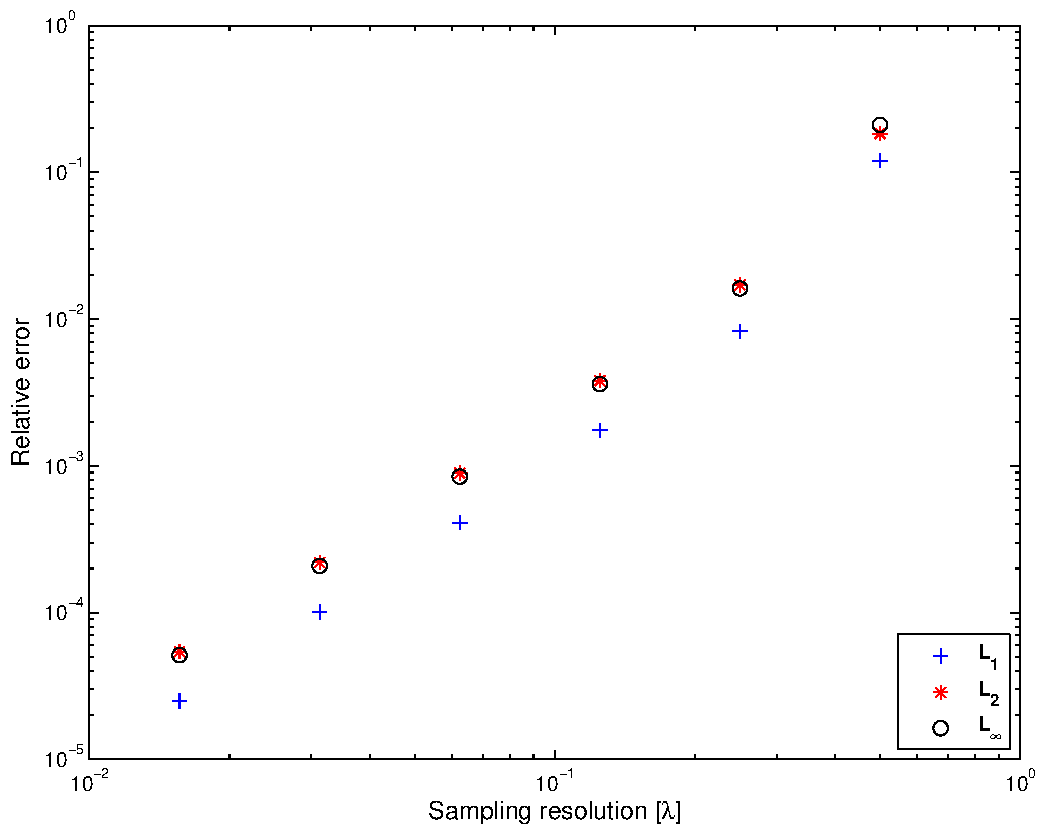
\includegraphics[width=12cm]{sph_error}
\caption{Relative broadside far field detector $\tilde{\psi}_r^*$ error in the $\mcal{L}^1$, $\mcal{L}^2$ and $\mcal{L}^\infty$ norms for several sampling resolutions.}
\label{fig:sph_error}
\end{figure}
We have chosen the $\mcal{L}^2$ norm or \itt{Euclidean norm} to compare the values of $\tilde{\psi}_{r \ \mrm{N2F}}^*$ and $\tilde{\psi}_{r \ \mrm{Direct}}^*$. This is motivated by the fact that the $\mcal{L}^2$ norm preserves energy information. Thus, the scalar N2F relative error will be given by the following relation\footnote{For \itt{Shannon's sampling theorem}, the lowest sampling resolution that can be used equals $\nicefrac{\lambda}{2}$.}
\begin{eqnarray}
\label{eq:errorScal}
\varepsilonup_{[\nicefrac{\lambda}{n}]} & = & \frac{\|\tilde{\psi}_{r \ \mrm{Direct}}^* - \tilde{\psi}_{r \ \mrm{N2F}}^* \|_2}{\| \tilde{\psi}_{r \ \mrm{Direct}}^* \|_2} \qquad n \in \mathbb{N}^{+} / \{ 1 \}.
\end{eqnarray}

\par As we can see in figures \ref{fig:sph3x5_Phi0_0_0} and \ref{fig:sph3x5_Phi90_0_0}, the sampling resolution of $\nicefrac{\lambda}{10}$ with an error of $\varepsilonup_{[\nicefrac{\lambda}{10}]} = 2.398 \ 10^{-3}$ for 181 \itt{look angles} ($\Delta \theta_r = 1$\�), that is the far zone directions in which $\tilde{\psi}_{r \ \mrm{N2F}}^*$ and $\tilde{\psi}_{r \ \mrm{Direct}}^*$ are computed, provides a pattern that can be considered reasonably accurate. As we can see in figure \ref{fig:sph_dTerror}, the number of look angles chosen does not significantly modify the error order even if the pattern is coarsely sampled (low number of look angles). However, there is a converging behavior while increasing the pattern sampling resolution ($\Delta \theta_r \rightarrow 0$).
\begin{figure}[!tbp]
\centering
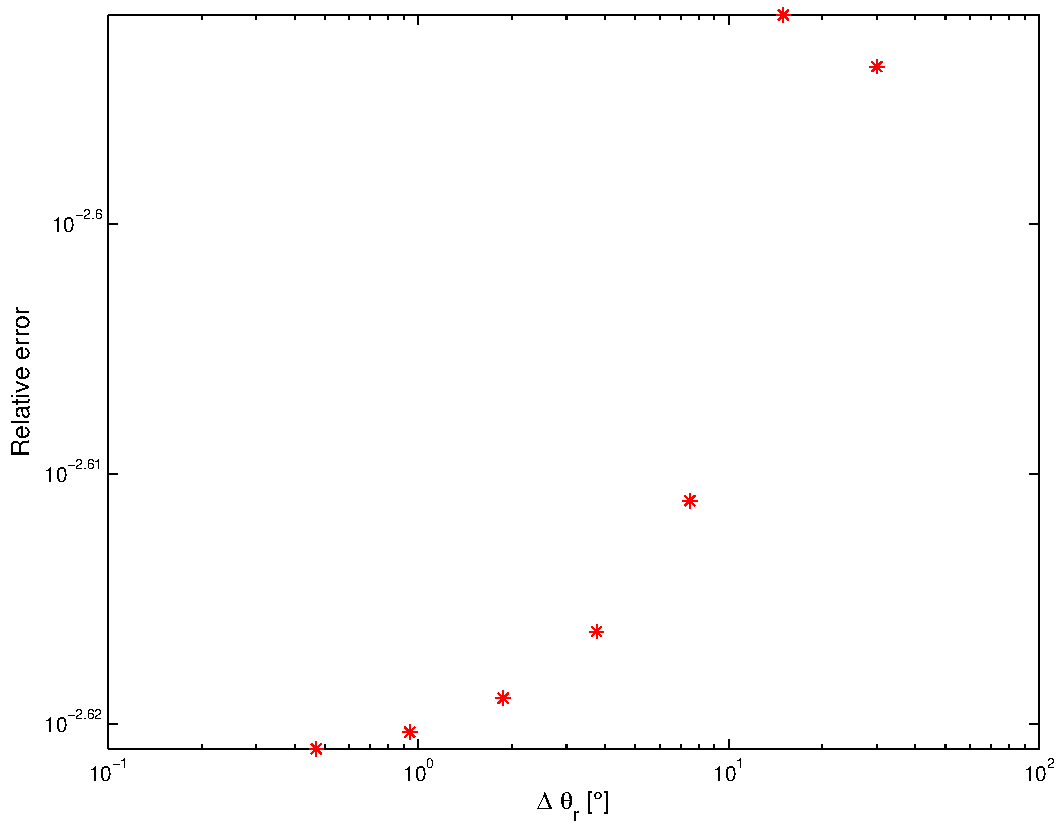
\includegraphics[width=12cm]{sph_dTerror}
\caption{Relative broadside far field detector pattern $\tilde{\psi}_r^*$ error in the $\mcal{L}^2$ norm for several $\Delta \theta_r$, i.e. increasing the pattern resolution.}
\label{fig:sph_dTerror}
\end{figure}
In order to define an accuracy criterion for the pattern computation, we will assume error values $\varepsilonup_{[\nicefrac{\lambda}{n}]} \leq 5 \ 10^{-3}$ to be admissible, and the integer $n$ will be consequently defined for the employed bounding surface. To motivate this choice, an example of pattern resulting in a higher error value ($\varepsilonup_{[\nicefrac{\lambda}{3}]} ~= ~3.387 \ 10^{-2}$) is given in figure \ref{fig:sph3x5_Phi90_0_0_lambda3}, showing a sensible misfit comparing to the reference pattern (directly computed), especially in the side lobes.
\begin{figure}[!tbp]
\centering
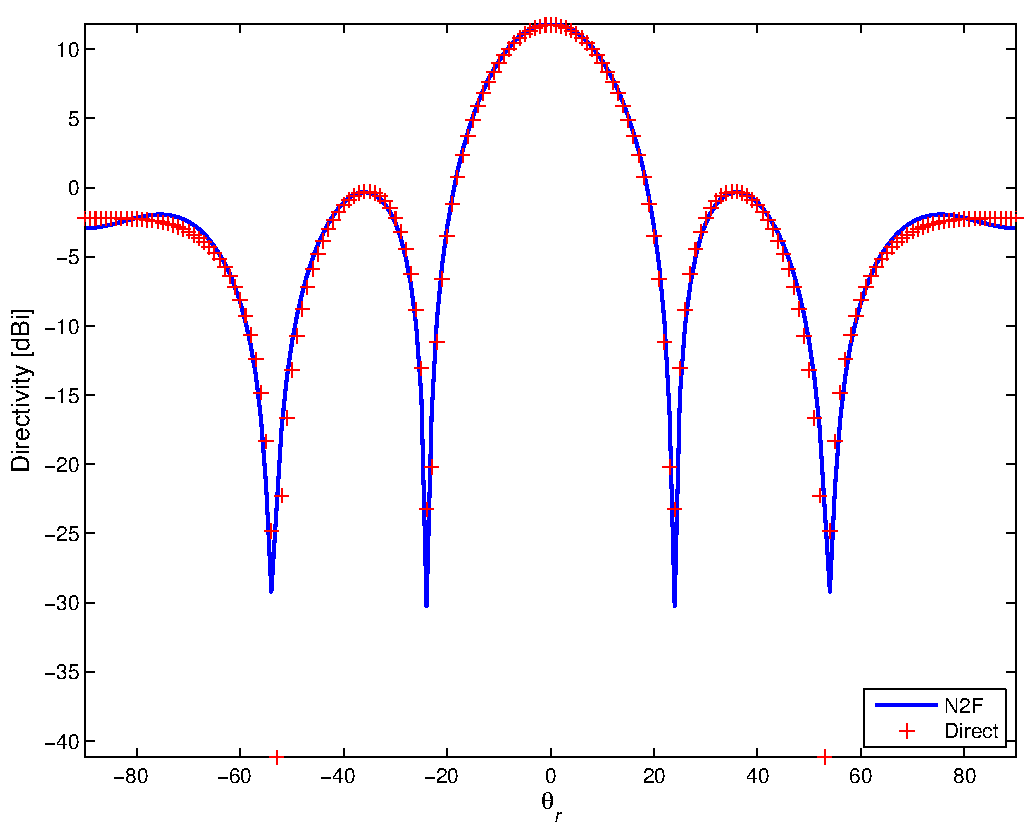
\includegraphics[width=12cm]{sph3x5_Phi90_0_0_lambda3}
\caption{Pattern computed on the $\phi=90$\textdegree \ cut plane with $\nicefrac{\lambda}{3}$ sampling resolution. Notice the visible error on the side lobes.}
\label{fig:sph3x5_Phi90_0_0_lambda3}
\end{figure}

\par Before we proceed with the N2F computations from a parallelepiped, let us face the steering operation, choosing opportunely the phase of $\tilde{S}_n, n = 1 \ldots N$, such that the main lobe in the pattern results in a desired direction. For a planar array with arbitrarily spaced sources, the phase values are  $\phiup _n = - k ( x_n \sin(\theta_{x}) + y_n \sin(\theta_{y}))$ \cite{StutzmanThieleATD} where $(x_n,y_n)$ are the position coordinates of the $n^\mrm{th}$ source, $\theta_x$ and $\theta_y$ are, respectively, the \itt{scan angles} along the $x$ and $y$ directions. Considering also the power normalization (see section \ref{sec:CompSteps}), the sources phasors become
\begin{eqnarray}
\label{eq:Excitations}
\tilde{S}_n = \frac{4\pi}{\sqrt{N}} \ \mrm{e}^{-jk ( x_n \sin(\theta_{x}) + y_n \sin(\theta_{y}))} \qquad n = 1 \ldots N
\end{eqnarray}
Figures \ref{fig:sph3x5_Phi0_10_30} and \ref{fig:sph3x5_Phi90_10_30} show the patterns on the cut planes XZ and YZ resulting from the steering operation of $\theta_x=10$\� \ and $\theta_y=30$\�.
\begin{figure}[!htbp]
\centering
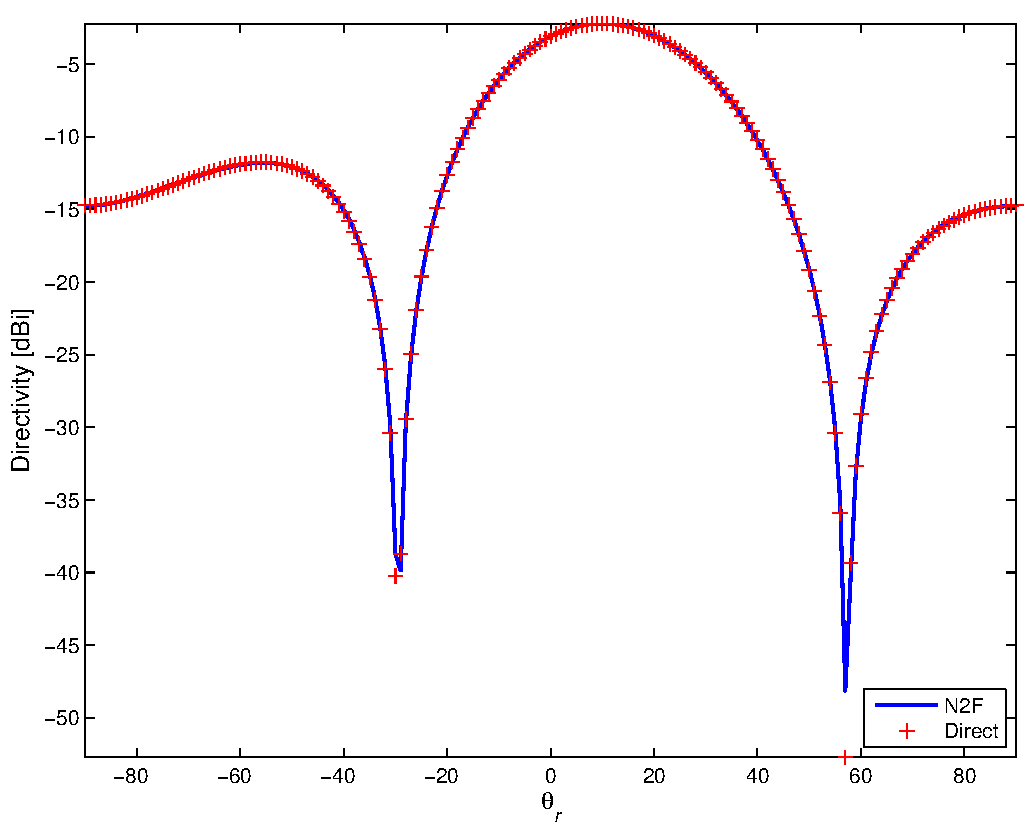
\includegraphics[width=12cm]{sph3x5_Phi0_10_30}
\caption{Pattern computed on the $\phi=0$\� \ cut plane with $\nicefrac{\lambda}{10}$ sampling resolution and scan angles $\theta_x=10$\� \ and $\theta_y=30$\�.}
\label{fig:sph3x5_Phi0_10_30}
\end{figure}
\begin{figure}[!htbp]
\centering
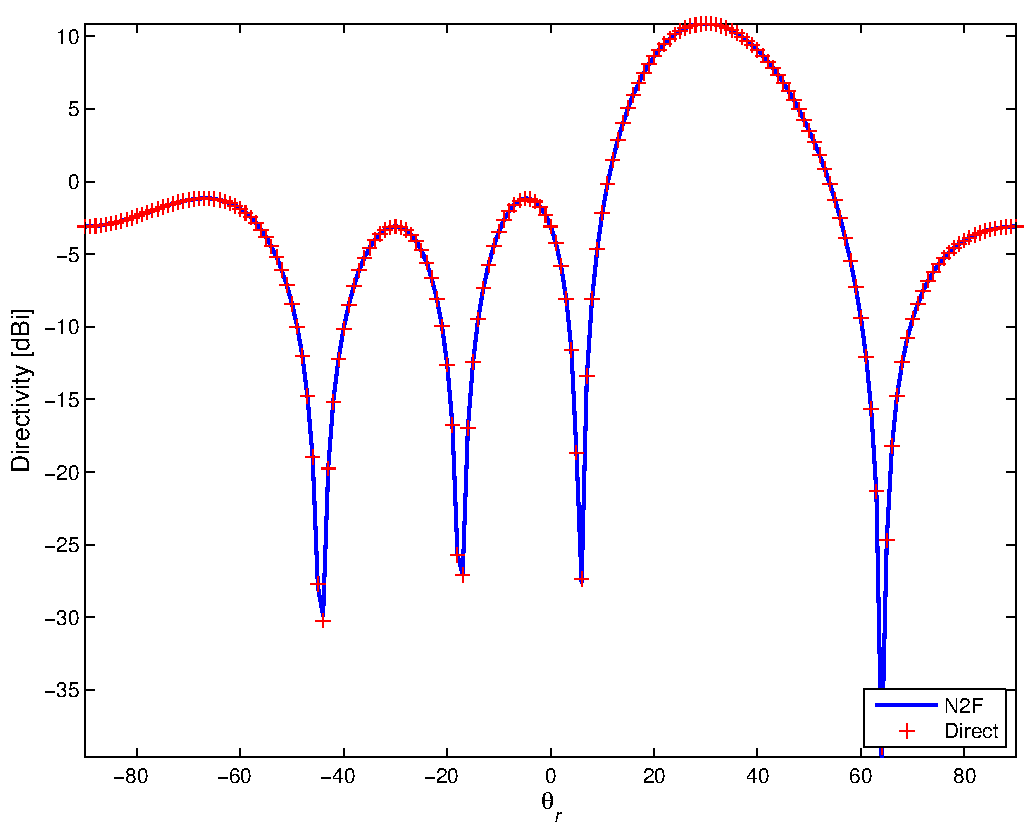
\includegraphics[width=12cm]{sph3x5_Phi90_10_30}
\caption{Pattern computed on the $\phi=90$\� \ cut plane with $\nicefrac{\lambda}{10}$ sampling resolution and scan angles $\theta_x=10$\� \ and $\theta_y=30$\�.}
\label{fig:sph3x5_Phi90_10_30}
\end{figure}


\subsection{Computations on a bounding parallelepiped} \label{sec:scalarBox}

\par The N2F computation on a bounding parallelepiped or box is achieved similarly to the one from a bounding sphere. Figure \ref{fig:box3x5} shows the mesh realized for the array of 3 by 5 point sources, with a resolution of $\nicefrac{\lambda}{10}$. The minimum distance between a point source and a surface patch is of $\nicefrac{\lambda}{2}$.

\begin{figure}[!tbp]
\centering
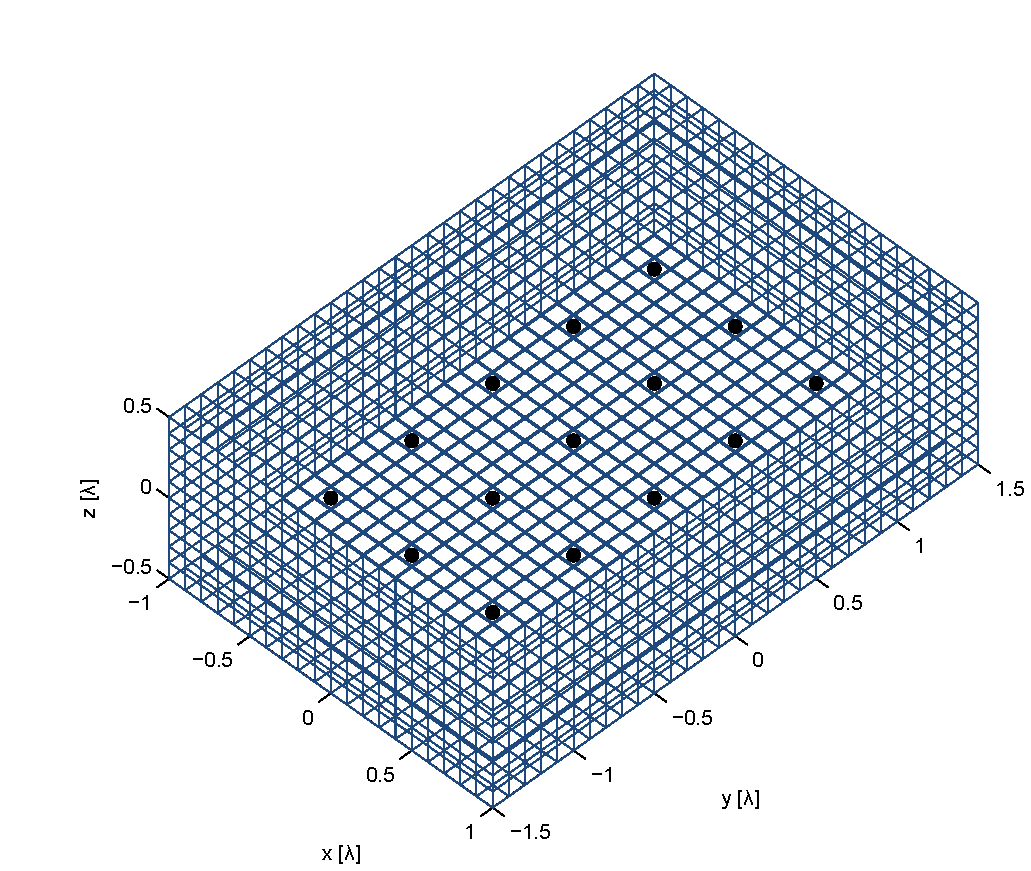
\includegraphics[width=12cm]{box3x5}
\caption{N2F bounding parallelepiped and 3 by 5 point sources, with $\nicefrac{\lambda}{10}$ sampling resolution.}
\label{fig:box3x5}
\end{figure}

\par The main difference between the two kinds of sampling geometries resides in the fact that the box requires a lower number of samples to achieve the same error as sphere's one. The box is in fact a closer encompassing surface. As we get far away from the point sources, we need a higher number of near field sampling points to keep the accuracy desired. In effect, the sphere surface patches ($\Delta S_m$) become larger as we increase the sphere radius, especially for the equatorial ones, leading to a coarse integration of the near fields and their derivatives. Furthermore, as we get away from the sources, the fields present higher structure, until they behave like the radiation patterns, that is varying rapidly of several orders of magnitude. Thus, we need to lower the dimension of the sphere patches for an accurate integration\footnote{A triangulated sphere, where the surface patches are composed of triangles of equal size, have also been used for better numerical integration. Nevertheless, this kind of discretization approach leads to higher computational requirements.}.
\begin{figure}[!htbp]
\centering
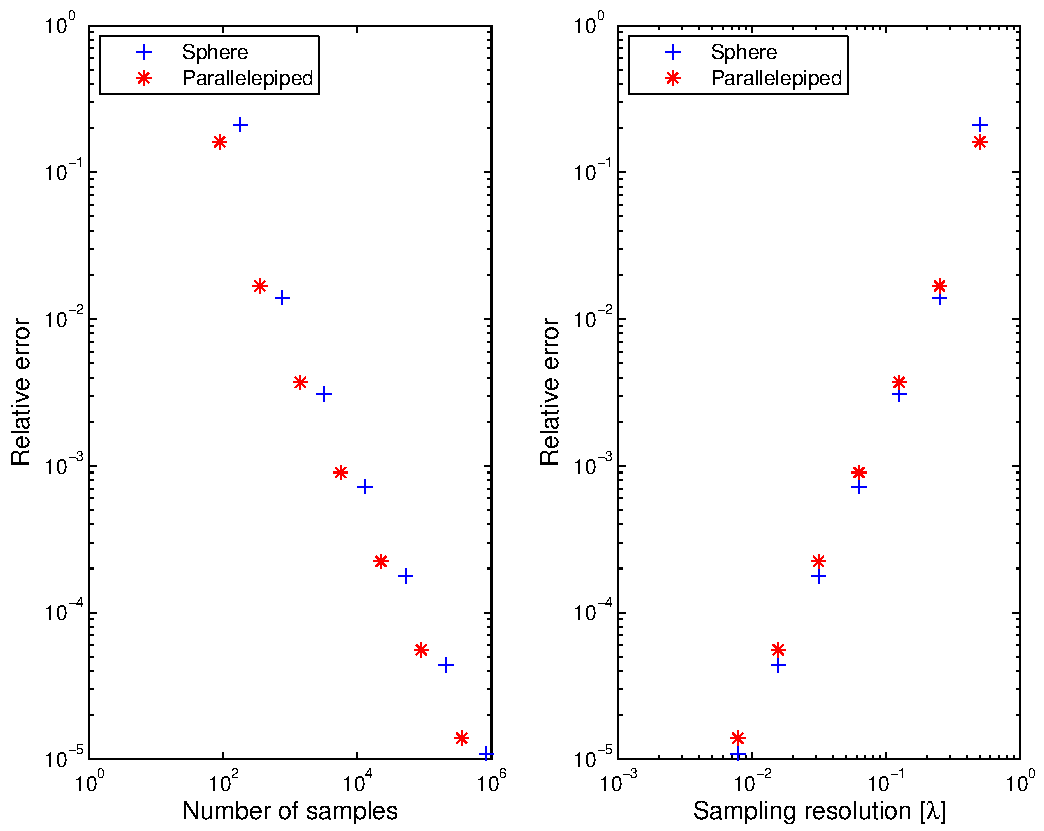
\includegraphics[width=14cm]{sphboxSampling}
\caption{Near fields sampling points comparisons between the one required by the sphere and those for the parallelepiped for the 3 by 5 point sources array.}
\label{fig:sphboxSampling}
\end{figure}
In figure \ref{fig:sphboxSampling} and table \ref{tab:sphboxSampling}, it is shown the improvement we obtain using a bounding box. In the average and for the chosen array, the box needs about half of the sphere's number of sampling points, thus halving the memory requirements while keeping the same error level.
\begin{table}[!htbp]
\centering
\begin{tabular}{|c|c|c|c|c|}
\hline Resolution & Sphere samples & Sphere error & Box samples & Box error \\
\hline \hline $\nicefrac{\lambda}{2}$ & 180 & $2.11 \ 10^{-1}$ & 88 & $1.61 \ 10^{-1}$ \\
\hline $\nicefrac{\lambda}{4}$ & 760 & $1.4 \ 10^{-2}$ & 352 & $1.68 \ 10^{-2}$ \\
\hline $\nicefrac{\lambda}{8}$ & 3 159 & $3.09 \ 10^{-3}$ & 1 408 & $3.71 \ 10^{-3}$ \\
\hline $\nicefrac{\lambda}{16}$ & 12 960 & $7.24 \ 10^{-4}$ & 5 632 & $9.01 \ 10^{-4}$ \\
\hline $\nicefrac{\lambda}{32}$ & 52 325 & $1.78 \ 10^{-4}$ & 22 528 & $2.24 \ 10^{-4}$ \\
\hline $\nicefrac{\lambda}{64}$ & 210 600 & $4.39 \ 10^{-5}$ & 90 112 & $5.58 \ 10^{-5}$ \\
\hline $\nicefrac{\lambda}{128}$ & 844 349 & $1.09 \ 10^{-5}$ & 360 448 & $1.39 \ 10^{-5}$ \\
\hline
\end{tabular}
\caption{Plotted values of figure \ref{fig:sphboxSampling}.}
\label{tab:sphboxSampling}
\end{table}

\par An interesting issue, seeking for further sampling coarsening to reduce the memory requirements, is to see what may happen if we omit some of the faces of the box, keeping the ones we expect to have higher power. The near field sampled on the box in a broadside steering condition are plotted in figures \ref{fig:boxFields} and \ref{fig:planesFields}. 

\begin{figure}[!hbtp]
%\begin{minipage}[b]{0.5\linewidth} % A minipage that covers half the page
\centering
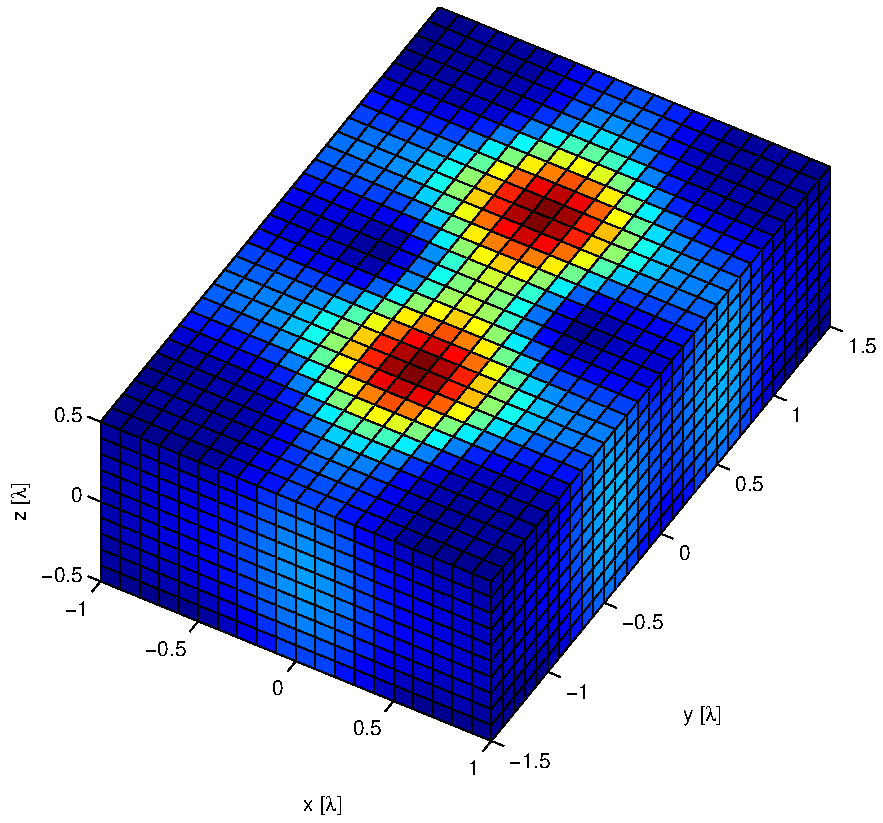
\includegraphics[width=10cm]{boxFields}
\caption{Near fields intensity $|\tilde{\psi}_m(\mbfit{r'}_m; \omega)|$ on the box with faces $\nicefrac{\lambda}{2}$ away from the point sources.}
\label{fig:boxFields}
%\end{minipage}
%\hspace{0.1cm} % To get a little bit of space between the figures
%\begin{minipage}[b]{0.5\linewidth}
\end{figure}
\begin{figure}[!hbtp]
\centering
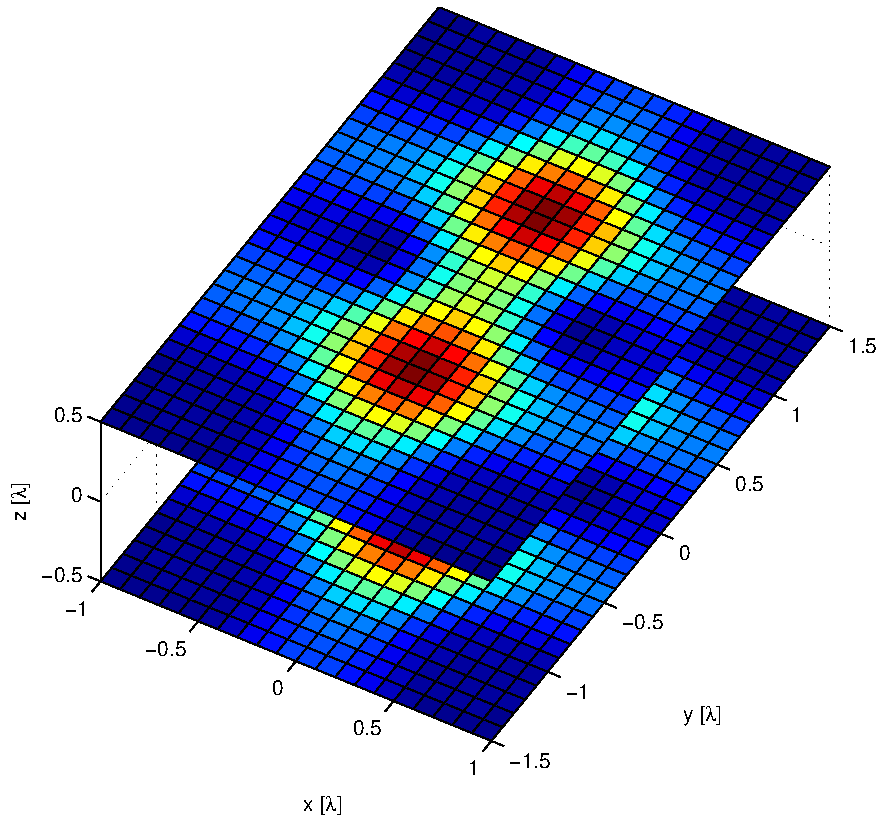
\includegraphics[width=10cm]{planesFields}
\caption{Near fields intensity on the top and bottom faces.}
\label{fig:planesFields}
%\end{minipage}
\end{figure}

\par We can see that the highest intensities are located on the top and bottom faces. To avoid significant disturbance in the remotion of the lateral faces, we prefer to further reduce the fields intensities on those faces increasing the top and bottom planes dimensions as shown in figure \ref{fig:planesFieldsExt25}. The omitted edge faces of the box have been set to lie $2.5 \lambda$ away from the point sources located at the corners of the array. The patterns computed from the two planes are depicted in figures \ref{fig:planes3x5_Phi0_0_0_ext25} and \ref{fig:planes3x5_Phi90_0_0_ext25}. The main lobe results to be accurately matched, and the error grows as we move to \itt{end fire} ($\pm$ 90\�) look angles : the total pattern error is of $\varepsilonup_{[\nicefrac{\lambda}{10}]} = 0.214$. It is clear that with this configuration, the scan angles will be restricted to a lower range around the broadside direction in order to preserve the main lobe accuracy, and an increase in the planes dimensions results into a wider range. However this increases the memory requirements, leading into a less numerically efficient configuration, especially for very large arrays (50 by 50 radiating elements for example).

\begin{figure}[!tbp]
\centering
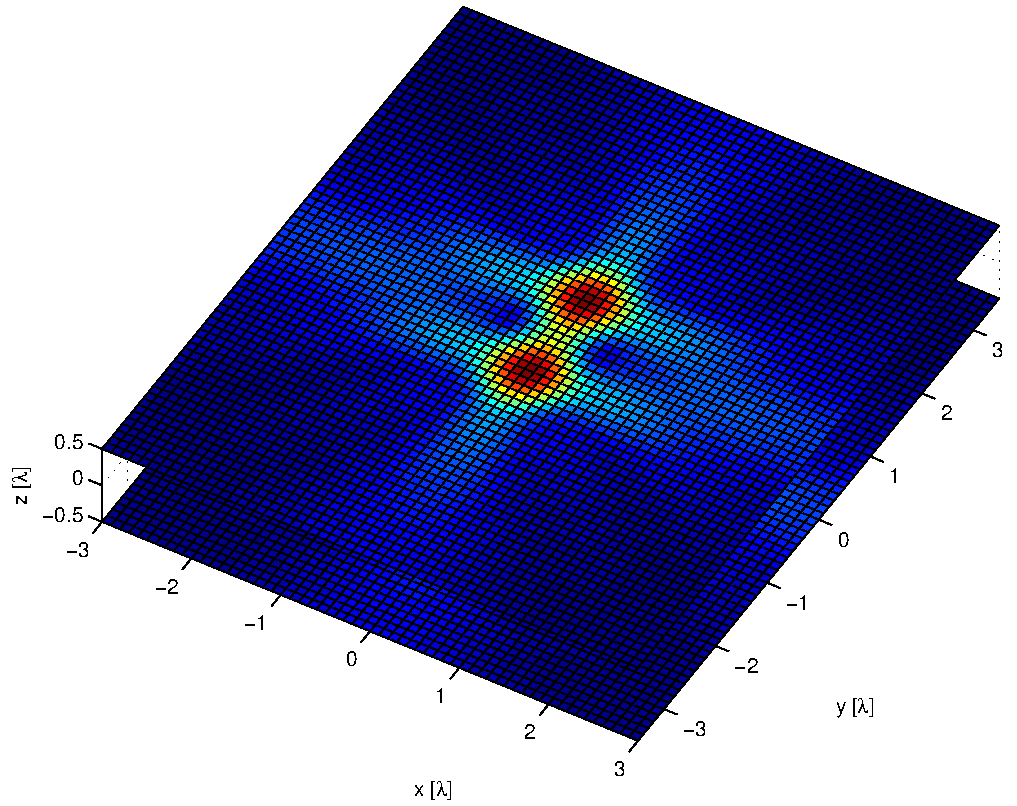
\includegraphics[width=14cm]{planesFieldsExt25}
\caption{Top and bottom planes for truncated surface computation. Lateral extension from the edge point sources is set to $2.5 \lambda$.}
\label{fig:planesFieldsExt25}
\end{figure}

\begin{figure}[!tbp]
\centering
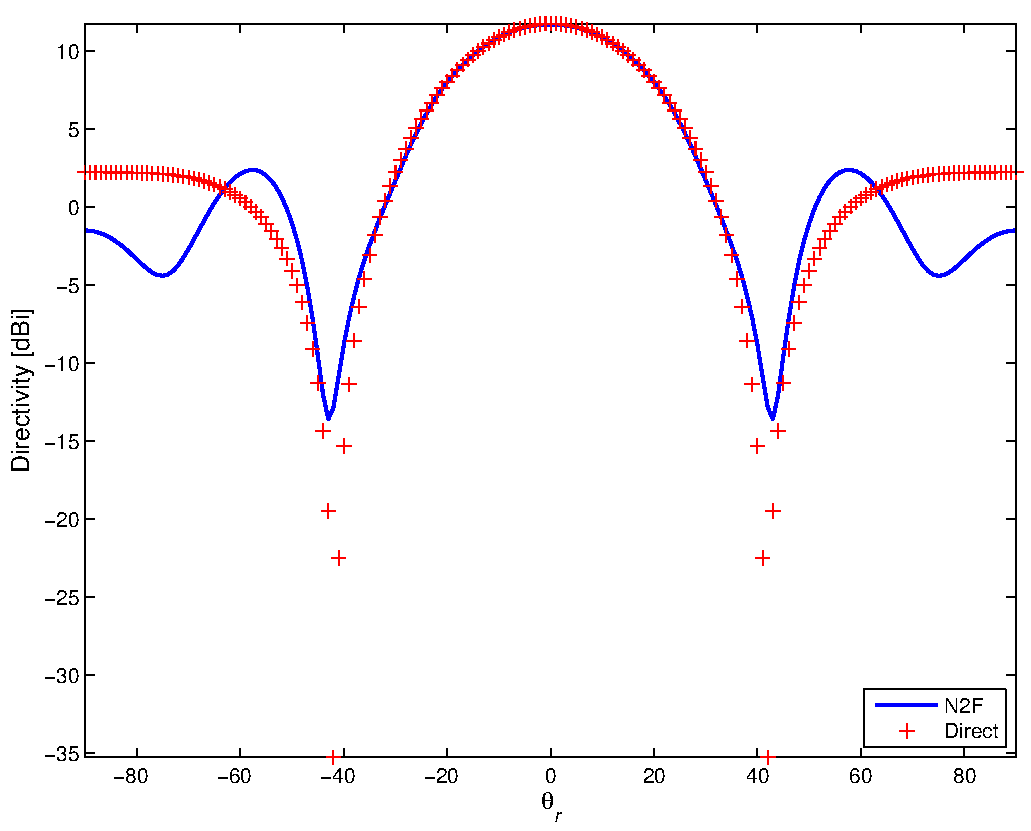
\includegraphics[width=12cm]{planes3x5_Phi0_0_0_ext25}
\caption{Pattern computed from the top and bottom faces of the box on the $\phi=0$\� \ cut plane ($\nicefrac{\lambda}{10}$ sampling resolution).}
\label{fig:planes3x5_Phi0_0_0_ext25}
\end{figure}
\begin{figure}[!tbp]
\centering
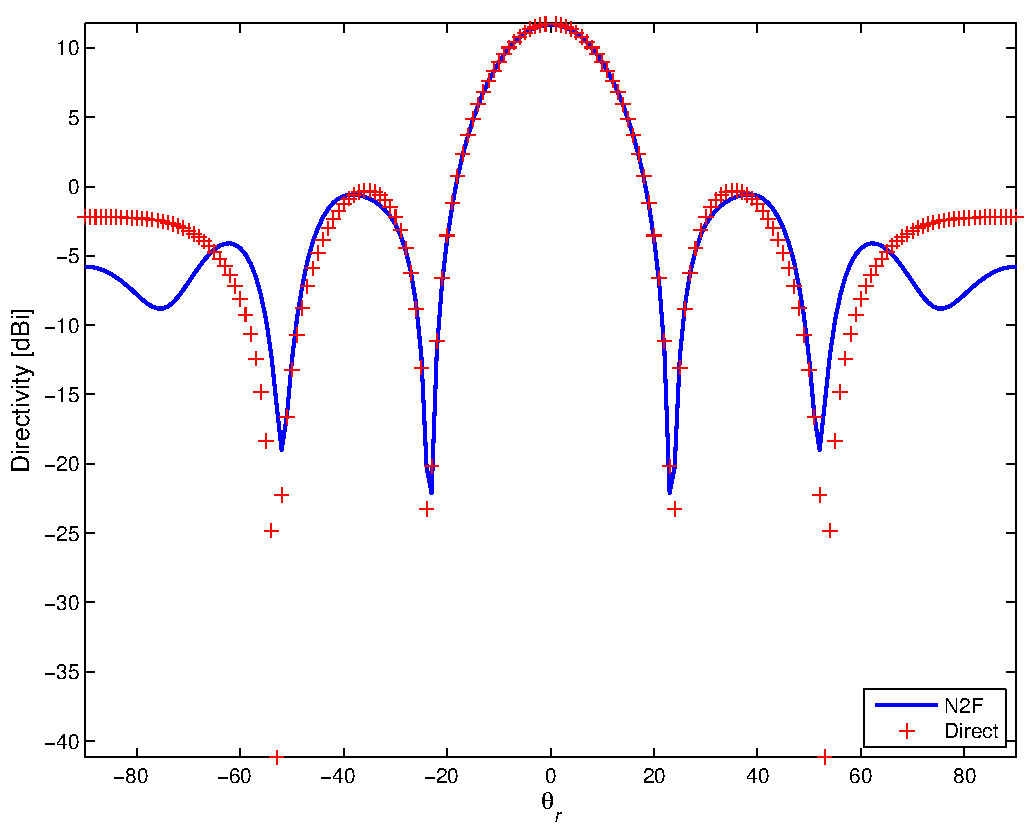
\includegraphics[width=12cm]{planes3x5_Phi90_0_0_ext25}
\caption{Pattern computed from the top and bottom faces of the box on the $\phi=90$\� \ cut plane ($\nicefrac{\lambda}{10}$ sampling resolution).}
\label{fig:planes3x5_Phi90_0_0_ext25}
\end{figure}



\newpage
%%%%%%%%%%%%%%%%%%%%%%%%%%%%%%%%%%%%%%%%%%%%%%%%%%%%%%%%%%%%%%%%%%%%%%%%%%%%%%%%%%%
\section{Vector near fields to far fields transformations} \label{sec:VectorN2F}

\par In this section, we present a numerical implementation of the vector near fields to far fields transformations (vector N2F), relying on the mathematical formulation discussed in section \ref{sec:VectorHuygens}. The computation steps are the same as discussed in section \ref{sec:CompSteps}. The results of an implementation in Matlab environment will be shown, considering as enclosing surface a parallelepiped. These results will be compared to ones obtained by means of the commercial CAD FEKO\footnote{FEKO${}^{\copyright}$ EM Software \& Systems. Further informations available on \url{www.feko.info}.}.

\subsection{Direct computation of the fields from current sources}

\par The Kottler's formulas (\ref{eq:KottlerE}-\ref{eq:KottlerH}) contains informations on both direct fields computations (first integral) and on N2F fields computations (second integral). To numerically evaluate the vector N2F, we have chosen to enclose an array of 3 by 5 \itt{Huygens' sources} \cite{MilliganMAD} with a box, in a similar manner as it has been done in section \ref{sec:scalarBox}. 
\begin{figure}[!tbp]
\centering
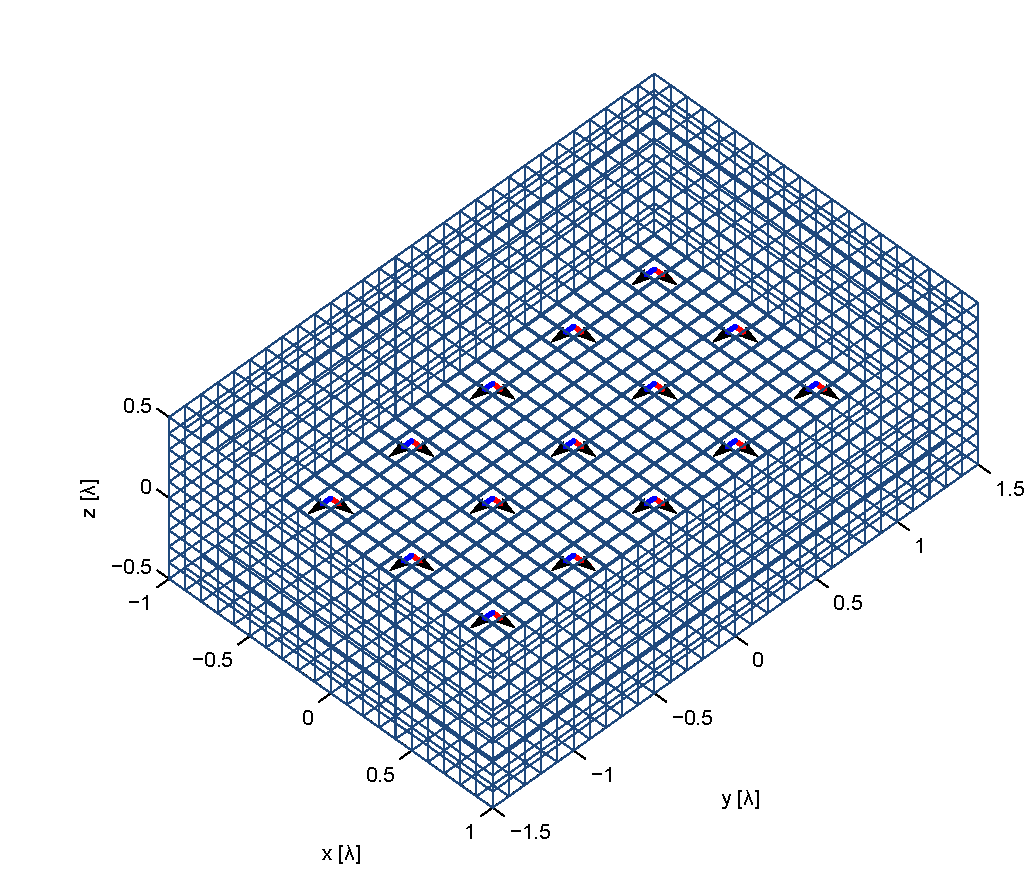
\includegraphics[width=12cm]{box3x5Vect}
\caption{N2F bounding parallelepiped and 3 by 5 Huygens' sources, with $\nicefrac{\lambda}{10}$ sampling resolution.}
\label{fig:box3x5Vect}
\end{figure}
Huygens' sources are made of an infinitesimal electric current $\tilde{\mbfit{J}}(\mbfit{r'}; \omega)$ crossing perpendicularly an infinitesimal magnetic current $\tilde{\mbfit{J}}_m(\mbfit{r'}; \omega)$. The amplitude of the magnetic current has to be $\zeta$ times bigger to achieve the same radiated power than the electric one. Hugens' sources are constructed as if they where derived from radiated fields (local plane wave behavior) and applying the equivalence principle (analog to Huygens' principle with equivalent currents, from which the name given to the sources). Now, to build the array, we have chosen the electric currents to be directed in $-\hat{\mbfit{y}}$ and the magnetic ones in $\hat{\mbfit{x}}$, such that the main radiation lobe is to be $\hat{\mbfit{z}}$-directed. Thus, we can express the currents of the array as
\begin{eqnarray}
\tilde{\mbfit{J}}(\mbfit{r'}; \omega) & = & - \tilde{J} \delta(\mbfit{r}-\mbfit{r'}) \hat{\mbfit{y}} \\
\tilde{\mbfit{J}}_m(\mbfit{r'}; \omega) & = & \zeta \tilde{J}_m \delta(\mbfit{r}-\mbfit{r'}) \hat{\mbfit{x}}
\end{eqnarray} where $\delta(\mbfit{r}-\mbfit{r'})$ is the Dirac delta, with its well known sifting property of integrals.

\par Let us now express analytically the terms involved with the Green's function \eqref{eq:GrFunc} in the first integrals of Kottler's equations. Using the relation 
\begin{eqnarray}
\label{eq:GradGreen}
\nabla G(\mbfit{r}|\mbfit{r'};\omega) = -{\nabla}' G(\mbfit{r}|\mbfit{r'};\omega) = \hat{\mbfit{R}} \frac{\partial}{\partial R} G(R;\omega),
\end{eqnarray} with $$G(\mbfit{r}|\mbfit{r'};\omega) = \frac{\mrm{e}^{-jk|\mbfit{r}-\mbfit{r'}|}}{4\pi|\mbfit{r}-\mbfit{r'}|} = \frac{\mrm{e}^{-jkR}}{4\pi R} = G(R;\omega),$$ we have
\begin{eqnarray}
\label{eq:GrGrad}
{\nabla}' G(\mbfit{r}|\mbfit{r'};\omega) = \left ( jk + \frac{1}{R} \right )  \frac{\mrm{e}^{-jkR}}{4\pi R} \hat{\mbfit{R}}.
\end{eqnarray} We need now to express explicitly the local gradient of \eqref{eq:GrGrad} \cite{VBladelSEFS}, that is the gradient of a vector-valued function of R. To do this, we express in spherical components the gradient operator to evaluate $\nabla A_R(R) \hat{\mbfit{R}}$, $A_R$ being the radial component of a vector-valued function $\mbfit{A}$ of R, where the transverse components $A_\theta$ and $A_\phi$ are null. We obtain
\begin{eqnarray}
\label{eq:GradVect}
\nabla \mbfit{A}(R) &= & \left ( \hat{\mbfit{R}} \frac{\partial}{\partial R} + \hat{\mbfit{\theta}} \frac{1}{R} \frac{\partial}{\partial \theta} + \hat{\mbfit{\phi}} \frac{1}{R \sin(\theta)} \frac{\partial}{\partial \phi  }\right )  A_R \hat{\mbfit{R}}  \nonumber \\
&= & \hat{\mbfit{R}} \frac{\partial}{\partial R} {A}_R \hat{\mbfit{R}} + \hat{\mbfit{\theta}} \frac{1}{R} \frac{\partial}{\partial \theta} {A}_R \hat{\mbfit{R}}+ \hat{\mbfit{\phi}} \frac{1}{R \sin(\theta)} \frac{\partial}{\partial \phi} {A}_R \hat{\mbfit{R}} \nonumber \\
&= &\hat{\mbfit{R}}\hat{\mbfit{R}} \frac{\partial}{\partial R} {A}_R  + \hat{\mbfit{\theta}} \hat{\mbfit{\theta}} \frac{1}{R} {A}_R + \hat{\mbfit{\phi}} \hat{\mbfit{\phi}} \frac{1}{R} {A}_R,
\end{eqnarray} where we have made the substitutions $\displaystyle \frac{\partial \hat{\mbfit{R}}}{\partial \theta} = \hat{\mbfit{\theta}}$ and $\displaystyle \frac{1}{\sin(\theta)} \frac{\partial \hat{\mbfit{R}}}{\partial \phi} = \hat{\mbfit{\phi}}$. With the use of the \itt{identity dyadic} $\dyad{I} = \hat{\mbfit{R}}\hat{\mbfit{R}}  + \hat{\mbfit{\theta}} \hat{\mbfit{\theta}} + \hat{\mbfit{\phi}} \hat{\mbfit{\phi}} = \hat{\mbfit{x}}\hat{\mbfit{x}}  + \hat{\mbfit{y}} \hat{\mbfit{y}} + \hat{\mbfit{z}} \hat{\mbfit{z}}$ in both spherical and Cartesian components, \eqref{eq:GradVect} can be rewritten as
\begin{eqnarray}
\label{eq:GradVectDyad}
\nabla \mbfit{A}(R) &= & \hat{\mbfit{R}}\hat{\mbfit{R}} \frac{\partial}{\partial R} {A}_R  + \left ( \dyad{I} - \hat{\mbfit{R}}\hat{\mbfit{R}} \right ) \frac{1}{R} {A}_R.
\end{eqnarray} Now, $\mbfit{A}(R)$ is substituted by ${\nabla}' G(\mbfit{r}|\mbfit{r'};\omega)$ and using \eqref{eq:GradGreen} we can write
\begin{eqnarray}
\label{eq:GradGradGreen}
{\nabla}' {\nabla}' G(\mbfit{r}|\mbfit{r'};\omega) &= & - \left (\hat{\mbfit{R}}\hat{\mbfit{R}} \frac{\partial}{\partial R} + \left ( \dyad{I} - \hat{\mbfit{R}}\hat{\mbfit{R}} \right ) \frac{1}{R} \right ) \left ( jk + \frac{1}{R} \right )  \frac{\mrm{e}^{-jkR}}{4\pi R}.
\end{eqnarray}
Noting that $\tilde{\mbfit{J}} \cdot \dyad{I} = \tilde{\mbfit{J}}$, Kottler's equations for an unbounded medium can be rewritten as, with $G = G(R;\omega)$,
\begin{eqnarray}
\label{eq:KottlerEdirect}
\tilde{\mbfit{E}}(\mbfit{r}; \omega) &= & \frac{1}{j \omega \epsilon} \int_V \left [  \tilde{\mbfit{J}} \left ( k^2 - \frac{jk}{R} - \frac{1}{R^2} \right ) G + \left ( \tilde{\mbfit{J}} \cdot \hat{\mbfit{R}} \right ) \hat{\mbfit{R}} \left (- k^2 + \frac{3jk}{R} + \frac{3}{R^2} \right) G \ - \right. \nonumber \\
& & \hspace{.5cm} \left. j \omega \epsilon \tilde{\mbfit{J}}_m  \times \hat{\mbfit{R}} \left ( jk + \frac{1}{R} \right ) G \right ] dV' \nonumber \\
&= & \frac{\zeta k^2}{4 \pi} \int_V \left [  \tilde{\mbfit{J}} \left ( - \frac{j}{kR} - \frac{1}{k^2R^2} + \frac{j}{k^3R^3} \right )  + \left ( \tilde{\mbfit{J}} \cdot \hat{\mbfit{R}} \right ) \hat{\mbfit{R}} \left (\frac{j}{kR} + \frac{3}{k^2R^2} - \frac{3j}{k^3R^3} \right) - \right. \nonumber \\
& & \hspace{.5cm} \left. \frac{1}{\zeta} \ \tilde{\mbfit{J}}_m  \times \hat{\mbfit{R}} \left ( \frac{j}{kR} + \frac{1}{k^2R^2} \right ) \right ] \mrm{e}^{-jkR} dV',
\end{eqnarray}
\begin{eqnarray}
\label{eq:KottlerHdirect}
\tilde{\mbfit{H}}(\mbfit{r}; \omega) &= & \frac{1}{j \omega \mu} \int_V \left [ \tilde{\mbfit{J}}_m \left ( k^2 - \frac{jk}{R} - \frac{1}{R^2} \right ) G + \left ( \tilde{\mbfit{J}}_m \cdot \hat{\mbfit{R}} \right ) \hat{\mbfit{R}} \left (- k^2 + \frac{3jk}{R} + \frac{3}{R^2} \right) G \ + \right. \nonumber \\
& & \hspace{.5cm} \left. j \omega \mu \tilde{\mbfit{J}}  \times \hat{\mbfit{R}} \left ( jk + \frac{1}{R} \right ) G \right ] dV' \nonumber \\
&= & \frac{k^2}{4 \pi \zeta} \int_V \left [ \tilde{\mbfit{J}}_m \left ( - \frac{j}{kR} - \frac{1}{k^2R^2} + \frac{j}{k^3R^3} \right ) + \right. \nonumber \\
& & \hspace{.5cm} \left. \left ( \tilde{\mbfit{J}}_m \cdot \hat{\mbfit{R}} \right ) \hat{\mbfit{R}} \left (\frac{j}{kR} + \frac{3}{k^2R^2} - \frac{3j}{k^3R^3} \right) + \right. \nonumber \\
& & \hspace{1cm} \left. \zeta \ \tilde{\mbfit{J}}  \times \hat{\mbfit{R}} \left ( \frac{j}{kR} + \frac{1}{k^2R^2} \right ) \right ] \mrm{e}^{-jkR}  dV'.
\end{eqnarray}
We can now compute the fields on the bounding surface, integrating over the volume enclosed and using the sifting property of the Dirac delta. The integration is done considering each vector component separately in a Cartesian coordinates system. Also, using the far fields approximation of the Green's function by \eqref{eq:GrAppr}, one can compute the pattern directly from the sources distribution.

\subsection{Near fields to far fields computations}

\par The second integral term of Kottler's equations (\ref{eq:KottlerE}-\ref{eq:KottlerH}) can be straightforwardly obtained from  (\ref{eq:KottlerEdirect}-\ref{eq:KottlerHdirect}), assuming the current terms to be equivalent currents on the bounding surface, such that the volume integrals reduce into surface integrals. Thus, we have
\begin{eqnarray}
\label{eq:KottlerEeq}
\tilde{\mbfit{E}}(\mbfit{r}; \omega) &= & \frac{\zeta k^2}{4 \pi} \oint_{S_0} \left [  \tilde{\mbfit{J}}_s^{eq} \left ( - \frac{j}{kR} - \frac{1}{k^2R^2} + \frac{j}{k^3R^3} \right )  +  \right. \nonumber \\
& & \hspace{.5cm} \left. \left ( \tilde{\mbfit{J}}_s^{eq} \cdot \hat{\mbfit{R}} \right ) \hat{\mbfit{R}} \left (\frac{j}{kR} + \frac{3}{k^2R^2} - \frac{3j}{k^3R^3} \right) - \right. \nonumber \\
& & \hspace{.5cm} \left. \frac{1}{\zeta} \ \tilde{\mbfit{J}}_{ms}^{eq}  \times \hat{\mbfit{R}} \left ( \frac{j}{kR} + \frac{1}{k^2R^2} \right ) \right ] \mrm{e}^{-jkR} \ dS',
\end{eqnarray}
\begin{eqnarray}
\label{eq:KottlerHeq}
\tilde{\mbfit{H}}(\mbfit{r}; \omega) &= & \frac{k^2}{4 \pi \zeta} \oint_{S_0} \left [ \tilde{\mbfit{J}}_{ms}^{eq} \left ( - \frac{j}{kR} - \frac{1}{k^2R^2} + \frac{j}{k^3R^3} \right ) + \right. \nonumber \\
& & \hspace{.5cm} \left. \left ( \tilde{\mbfit{J}}_{ms}^{eq} \cdot \hat{\mbfit{R}} \right ) \hat{\mbfit{R}} \left (\frac{j}{kR} + \frac{3}{k^2R^2} - \frac{3j}{k^3R^3} \right) + \right. \nonumber \\
& & \hspace{1cm} \left. \zeta \ \tilde{\mbfit{J}}_s^{eq}  \times \hat{\mbfit{R}} \left ( \frac{j}{kR} + \frac{1}{k^2R^2} \right ) \right ] \mrm{e}^{-jkR} \ dS',
\end{eqnarray} where $\tilde{\mbfit{J}}_s^{eq} = \tilde{\mbfit{J}}_s^{eq}(\mbfit{r'}; \omega) = \hat{\mbfit{n}} \times \tilde{\mbfit{H}}(\mbfit{r'}; \omega)$ and $\tilde{\mbfit{J}}_{ms}^{eq} = \tilde{\mbfit{J}}_{ms}^{eq}(\mbfit{r'}; \omega) =- \hat{\mbfit{n}} \times \tilde{\mbfit{E}}(\mbfit{r'}; \omega)$. With the far fields approximation of the Green's function \eqref{eq:GrAppr}, the second integral term of Kottler's equations (\ref{eq:KottlerEeq}-\ref{eq:KottlerHeq}) become
\begin{eqnarray}
\label{eq:KottlerEN2Fapprox}
\hspace{-1cm} \tilde{\mbfit{E}}(\mbfit{r}; \omega) \Big|_{r \gg r'}  &\approx& j \zeta k \frac{\mrm{e}^{-jk r}}{4\pi r} \oint_{S_0}  \mrm{e}^{jk \hat{\mbfit{r}} \cdot \mbfit{r'}} \left [ - \tilde{\mbfit{J}}_s^{eq}  + \left ( \tilde{\mbfit{J}}_s^{eq} \cdot \hat{\mbfit{r}} \right ) \hat{\mbfit{r}} - \frac{1}{\zeta} \ \tilde{\mbfit{J}}_{ms}^{eq}  \times \hat{\mbfit{r}} \right ]  dS',
\end{eqnarray}
\begin{eqnarray}
\label{eq:KottlerHN2Fapprox}
\hspace{-1cm} \tilde{\mbfit{H}}(\mbfit{r}; \omega) \Big|_{r \gg r'} &\approx & j \frac{k}{\zeta} \frac{\mrm{e}^{-jk r}}{4\pi r} \oint_{S_0}  \mrm{e}^{jk \hat{\mbfit{r}} \cdot \mbfit{r'}} \left [ - \tilde{\mbfit{J}}_{ms}^{eq}  + \left ( \tilde{\mbfit{J}}_{ms}^{eq} \cdot \hat{\mbfit{r}} \right ) \hat{\mbfit{r}} + \zeta \ \tilde{\mbfit{J}}_{s}^{eq}  \times \hat{\mbfit{r}} \right ]  dS'.
\end{eqnarray}

\subsection{Radiation pattern}

\par With (\ref{eq:KottlerEN2Fapprox}-\ref{eq:KottlerHN2Fapprox}), we can now derive the far fields pattern. As the computations are done considering the Cartesian components of the currents $\tilde{\mbfit{J}}$ and $\tilde{\mbfit{J}}_m$, or $\tilde{\mbfit{J}}_s^{eq}$ and $\tilde{\mbfit{J}}_{ms}^{eq}$ in the vector N2F, and the Cartesian components of the unit vector $\hat{\mbfit{R}} \begin{array}[t]{c}  \approx \\[-15pt] \scriptstyle {r \gg r'}  \end{array} \hat{\mbfit{r}}$, the resulting far fields detectors $\tilde{\mbfit{E}}^{*}$ and $\tilde{\mbfit{H}}^{*}$ are in Cartesian components : $\tilde{\mbfit{E}}_x^{*}$, $\tilde{\mbfit{E}}_y^{*}$, $\tilde{\mbfit{E}}_z^{*}$ and $\tilde{\mbfit{H}}_x^{*}$, $\tilde{\mbfit{H}}_y^{*}$, $\tilde{\mbfit{H}}_z^{*}$. To simplify the pattern computations, these can be converted into spherical components\footnote{$\mbfit{A}_r = \mbfit{A}_x\sin(\theta)\cos(\phi) + \mbfit{A}_y\sin(\theta)\sin(\phi) + \mbfit{A}_z\cos(\theta)$, $\mbfit{A}_\theta = \mbfit{A}_x\cos(\theta)\cos(\phi) + \mbfit{A}_y\cos(\theta)\sin(\phi) - \mbfit{A}_z\sin(\theta)$ and $\mbfit{A}_\phi = -\mbfit{A}_x\sin(\phi) + \mbfit{A}_y\cos(\phi)$. \cite{BalanisAT} \label{fn:cart2sph}} and discard the radial components $\tilde{\mbfit{E}}_r^{*}$ and $\tilde{\mbfit{H}}_r^{*}$ which must be null in the far zones. Furthermore, the radiated fields behavior in the far zones, that is
\begin{eqnarray}
\tilde{\mbfit{H}}^* &= & \frac{1}{\zeta} \hat{\mbfit{r}} \times \tilde{\mbfit{E}}^*,
\end{eqnarray} allows us to keep either the electric field or the magnetic field to derive the directivity pattern of the radiating structure. We have chosen to keep the electric far field detectors $\tilde{\mbfit{E}}_\theta^{*}$ and $\tilde{\mbfit{E}}_\phi^{*}$ from which the directivity can be obtained in term of $\theta$ and $\phi$ polarizations by the following expressions \cite{MilliganMAD, RothwellCloudE}
\begin{eqnarray}
\mathcal{P}_\theta \left ( \hat{\mbfit{r}}; \omega \right ) &= & \lim_{r \to \infty} 4 \pi r^2 \frac{S_{r[\theta]}}{\mrm{P}_r} = 4 \pi \frac{\left | \tilde{\mbfit{E}}_\theta^{*} \right |^2}{2 \zeta \mrm{P}_r} = 2 \pi \frac{\left | \tilde{\mbfit{E}}_\theta^{*} \right |^2}{ \zeta \mrm{P}_r}, \label{eq:patternForm1} \\ 
\mathcal{P}_\phi \left ( \hat{\mbfit{r}}; \omega \right ) &= &  \lim_{r \to \infty} 4 \pi r^2 \frac{S_{r[\phi]}}{\mrm{P}_r} = 4 \pi \frac{\left | \tilde{\mbfit{E}}_\phi^{*} \right |^2}{2 \zeta \mrm{P}_r} = 2 \pi \frac{\left | \tilde{\mbfit{E}}_\phi^{*} \right |^2}{ \zeta \mrm{P}_r},\label{eq:patternForm2}
\end{eqnarray} where $S_{r[\theta]}$ and $S_{r[\phi]}$ are the active power densities related to each of the polarizations\footnote{Real part of the radial component of the \itt{Poynting vector}, the first due to $\theta$-polarized electric field and the second due to $\phi$-polarized electric field.}. The term ${\mrm{P}_r}$ is the radiated power that, for practical reasons, has to be computed from the fields on the bounding surface. In effect, we could compute the total power using the far fields detectors, selecting the appropriate number of look angles to cover a sphere, but this is excessively time consuming. The computation of the power radiated from the near fields is achieved by an integration of the flux of the Poynting vector and keeping half of the real part. In other terms
\begin{eqnarray}
\label{eq:Pr}
\mrm{P}_r &= & \frac{1}{2} \Re \left \{ \oint_{S_0} \mbfit{S}_r(\mbfit{r'};\omega) \cdot \hat{\mbfit{n}} \ dS' \right \} \nonumber \\
&= & \frac{1}{2} \Re \left \{ \oint_{S_0} \left [ \tilde{\mbfit{E}}(\mbfit{r'};\omega) \times \tilde{\mbfit{H}}^{\dagger}(\mbfit{r'};\omega) \right ] \cdot \hat{\mbfit{n}} \ dS' \right \}
\end{eqnarray} where the symbol $\dagger$ indicates the complex conjugate. The total directivity pattern, polarization independent, is given by
\begin{eqnarray}
\mathcal{P} \left ( \hat{\mbfit{r}}; \omega \right ) &= & \mathcal{P}_\theta \left ( \hat{\mbfit{r}}; \omega \right ) + \mathcal{P}_\phi \left ( \hat{\mbfit{r}}; \omega \right ).
\end{eqnarray}

\subsection{Numerical results} \label{sec:NumResChap1}

\par We proceed with the numerical implementation that computes the vector N2F on the array depicted in figure \ref{fig:box3x5Vect}, comparing it to results obtained with FEKO. All the surface integrals have been computed by means of numerical midpoint integrations for each vector component separately, in a similar manner as it was done for the scalar field in section \ref{sec:ScalarN2F} (see note \ref{fn:midPointInt}). 
Figure \ref{fig:boxNFvector} shows the power density on the box surface computed by our implementation. Notice that, as the sources are not radiating isotropically but mainly along the $\hat{\mbfit{z}}$ direction, the level of the fields on the lateral faces of the box is low when compared to those generated by point sources (figure \ref{fig:boxFields}). In order to compare our implementation results to FEKO's ones, the frequency of the sources has been set to 1 GHz in both simulation environments. Also, the electric currents are set to be of 1 $\mrm{[\nicefrac{\mrm A}{\mrm{m^2}}]}$ and the magnetic currents are of $\zeta_0 \approx 376.73$ $\mrm{[\nicefrac{\mrm V}{\mrm{m^2}}]}$. The FEKO model of the array analyzed is depicted in figure \ref{fig:FEKOgeom}.
\begin{figure}[!htbp]
\centering
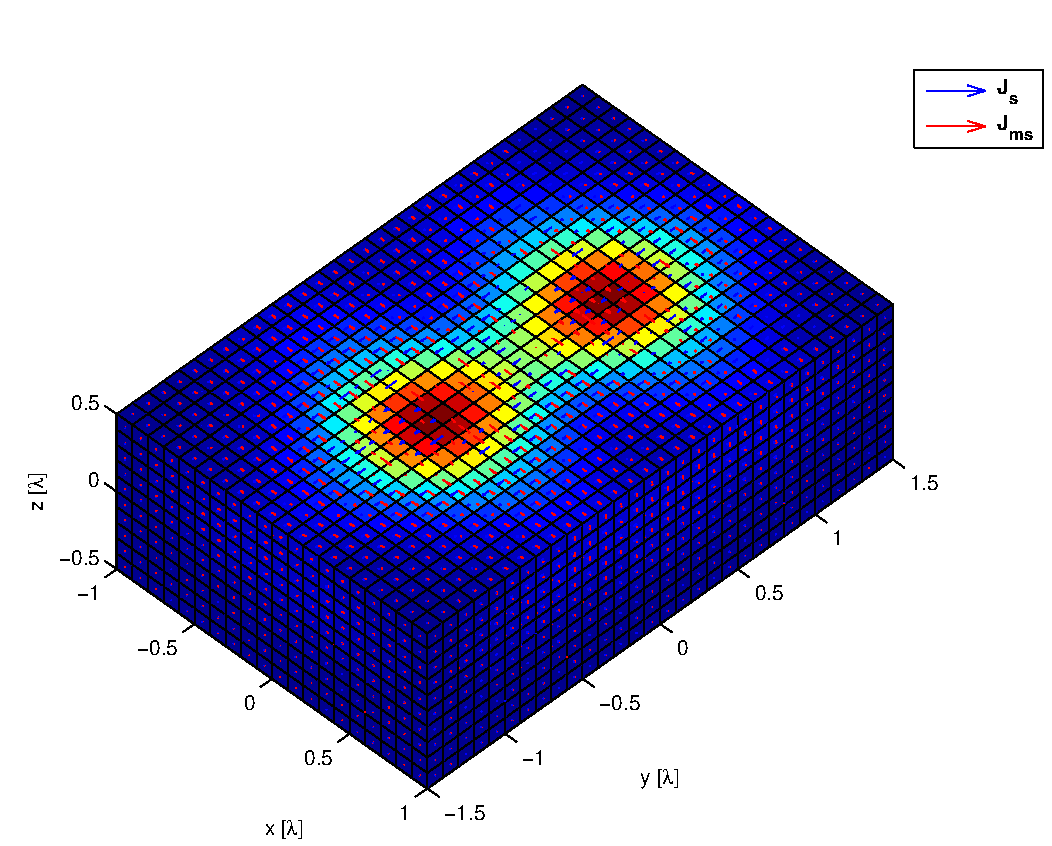
\includegraphics[width=12cm]{boxNFvector}
\caption{Surface power density and real part of the equivalent currents computed on the box of figure \ref{fig:box3x5Vect}.}
\label{fig:boxNFvector}
\end{figure} 
\begin{figure}[!htbp]
\centering
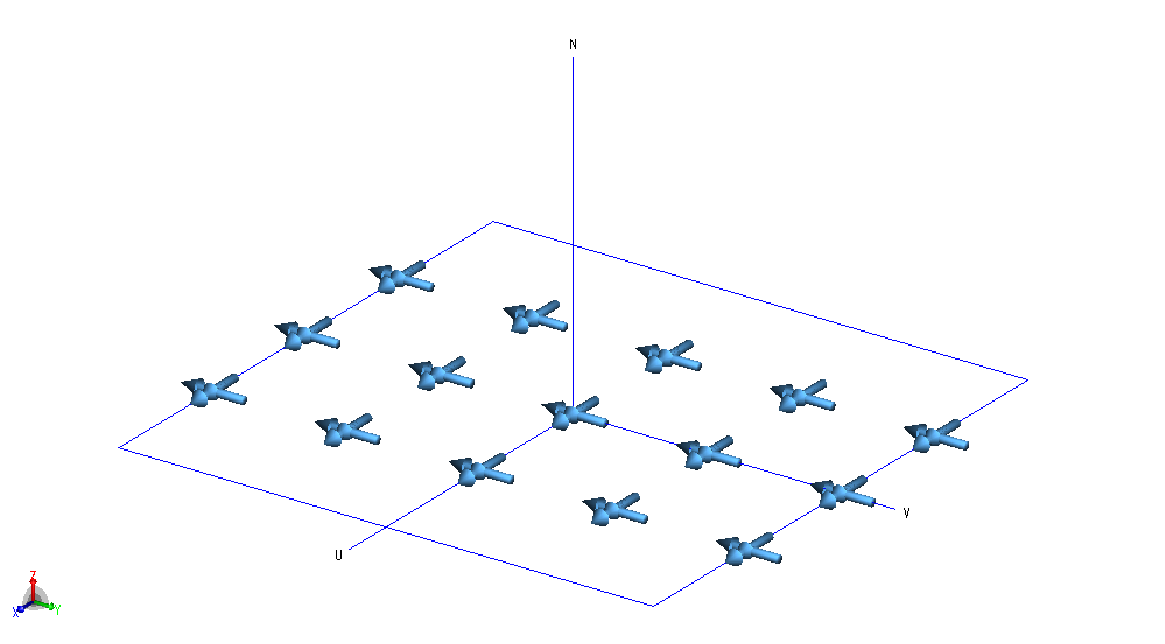
\includegraphics[width=12cm]{FEKOgeom}
\caption{FEKO model of the 3 by 5 Huygens' sources array of figure \ref{fig:box3x5Vect}.}
\label{fig:FEKOgeom}
\end{figure}
\par The patterns on the XZ and YZ cut planes computed with FEKO are shown in figures \ref{fig:FEKOPhi0} and \ref{fig:FEKOPhi90}. Both of them are the total fields directivity patterns (no polarization splitting) and they have a maximum value of $16.474$ [dBi] on the broadside direction. 
\begin{figure}[!htbp]
\begin{minipage}[b]{0.5\linewidth} % A minipage that covers half the page
\centering
\includegraphics[width=7.3cm]{FEKOPhi0}
\caption{Pattern computed with FEKO on the $\phi=0$\� \ cut plane.}
\label{fig:FEKOPhi0}
\end{minipage}
\hspace{0.1cm} % To get a little bit of space between the figures
\begin{minipage}[b]{0.5\linewidth}
\centering
\includegraphics[width=7.3cm]{FEKOPhi90}
\caption{Pattern computed with FEKO on the $\phi=90$\� \ cut plane.}
\label{fig:FEKOPhi90}
\end{minipage}
\end{figure}
\begin{figure}[!htbp]
\centering
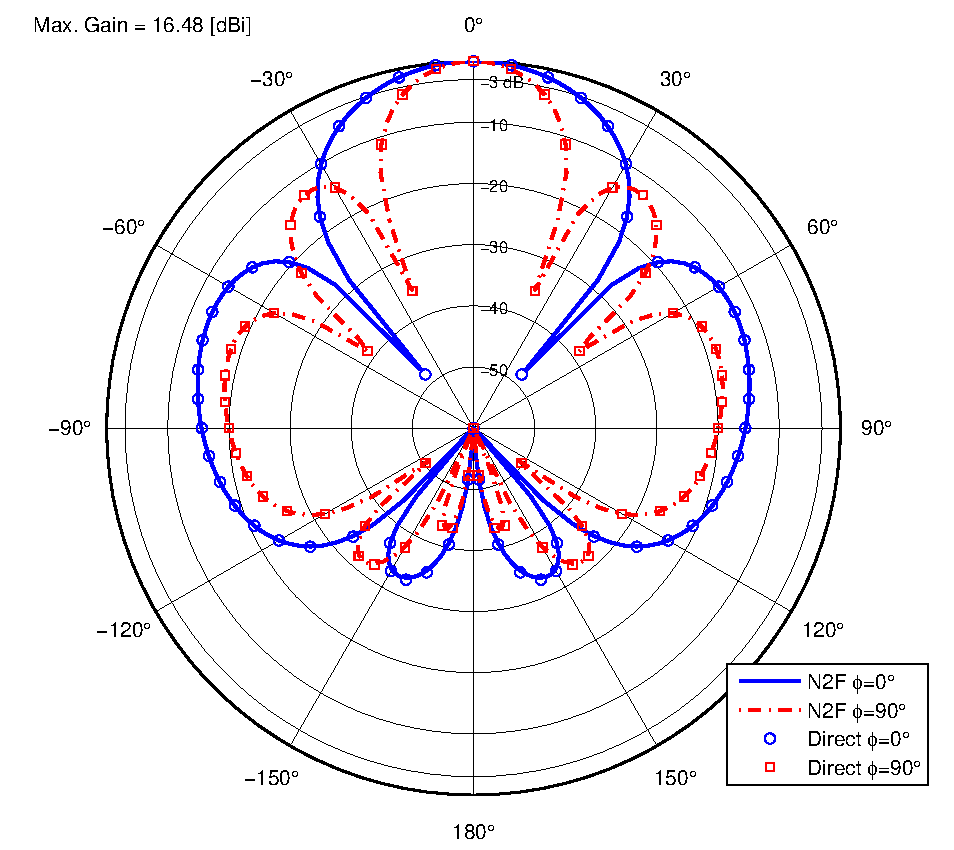
\includegraphics[width=12cm]{box3x5_0_0}
\caption{N2F and direct total fields directivity patterns computed for the array of figure \ref{fig:boxNFvector}.}
\label{fig:box3x5_0_0}
\end{figure}
The total power radiated by the array, for FEKO, is of $1.3346 \ 10^5$ [W], while our implementation gives $1.33528 \ 10^5$ [W] with $\nicefrac{\lambda}{10}$ of sampling resolution on the box, that is $-0.051$ \% of relative error. Notice that errors in the power radiated computation can vary sensibly to the maximum directivity, but not the pattern shape. The total pattern achieved with our implementation is depicted in figure \ref{fig:box3x5_0_0}. The maximum directivity achieved is of $16.481$ [dBi], slightly higher than the one computed by FEKO, and this is mainly due to the misfit in the power radiated computation(coarse integration of the power density on the box). In effect, as we will see below, the error on the fields detectors have resulted to be very low. However, for practical applications, that error can be considered to be low enough and the pattern sufficiently accurate.

\par The pattern formulation has been split into $\theta$ and $\phi$ polarizations, and this allows us to evaluate the co- and cross-polarizations amounts for real antennas. Plots of $  \mathcal{P}_\theta \left ( \hat{\mbfit{r}}; \omega \right ) $ and $ \mathcal{P}_\phi \left ( \hat{\mbfit{r}}; \omega \right )$ are given in figures \ref{fig:box3x5_0_0_1} and \ref{fig:box3x5_0_0_2}.
\begin{figure}[!htbp]
\begin{minipage}[b]{0.5\linewidth}
\centering
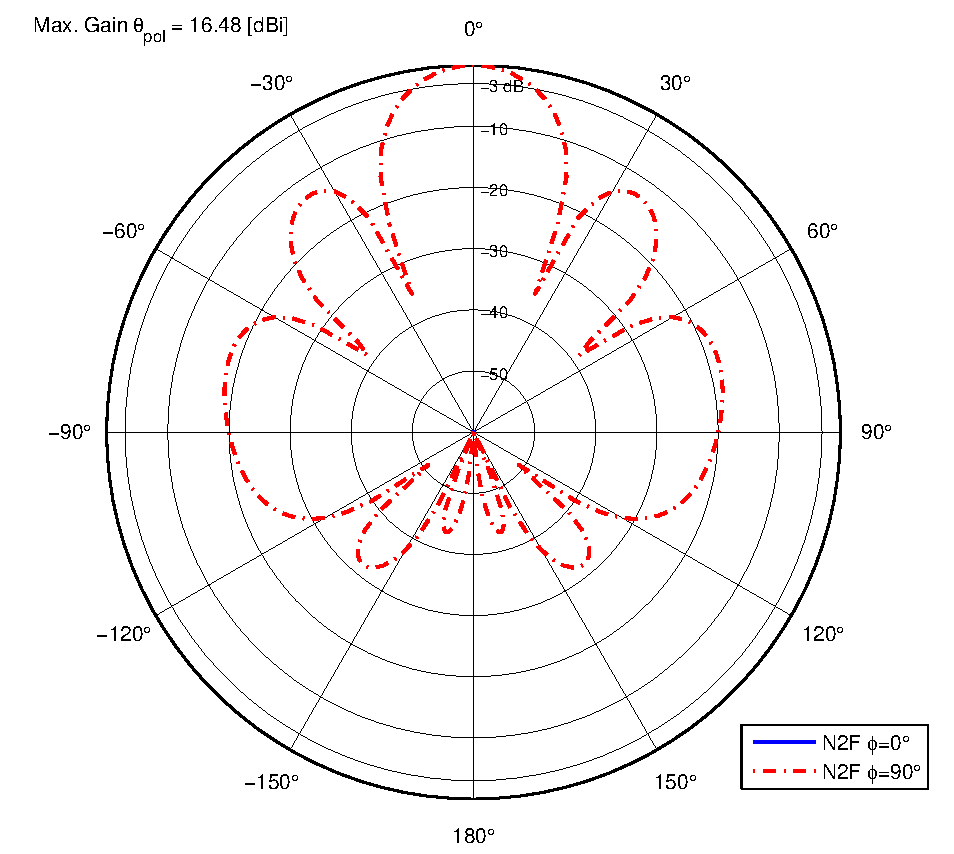
\includegraphics[width=7.3cm]{box3x5_0_0_1}
\caption{$\theta$ polarization pattern $\mathcal{P}_\theta \left ( \hat{\mbfit{r}}; \omega \right )$ of the 3 by 5 Huygens sources array.}
\label{fig:box3x5_0_0_1}
\end{minipage}
\hspace{0.1cm}
\begin{minipage}[b]{0.5\linewidth}
\centering
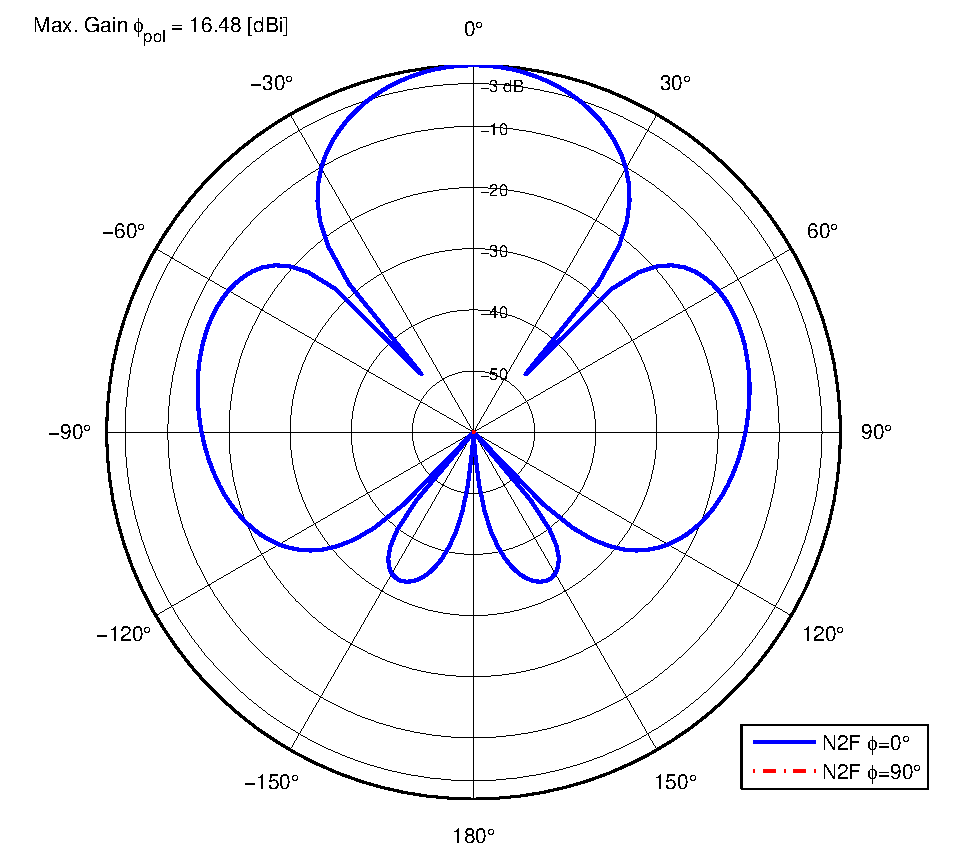
\includegraphics[width=7.3cm]{box3x5_0_0_2}
\caption{$\phi$ polarization pattern $\mathcal{P}_\phi \left ( \hat{\mbfit{r}}; \omega \right )$ of the 3 by 5 Huygens sources array.}
\label{fig:box3x5_0_0_2}
\end{minipage}
\end{figure}

\par Let us now quantify the error between the patterns computed by N2F and direct processes, using the following relation, similarly to \ref{eq:errorScal},
\begin{eqnarray}
\label{eq:errorVect}
\varepsilonup_{[\mrm{Direct-N2F}]} & = & \frac{\left  \| \left ( \tilde{\mbfit{E}}_{\mrm{Direct}\theta}^{*} + \tilde{\mbfit{E}}_{\mrm{Direct}\phi}^{*} \right ) - \left ( \tilde{\mbfit{E}}_{\mrm{N2F}\theta}^{*} + \tilde{\mbfit{E}}_{\mrm{N2F}\phi}^{*} \right ) \right \|_2}{\left  \| \tilde{\mbfit{E}}_{\mrm{Direct}\theta}^{*} + \tilde{\mbfit{E}}_{\mrm{Direct}\phi}^{*} \right \|_2}.
\end{eqnarray}
The FEKO results have been compared first to those of the direct computation using \eqref{eq:errorVect}. The error in this case is of $\varepsilonup_{[\mrm{Direct-FEKO}]} = 1.487 \ 10^{-4}$, which significantly validates our implementation. Then, comparing them to the N2F results, we have $\varepsilonup_{[\mrm{N2F \ [\nicefrac{\lambda}{10}]-FEKO}]} = 1.821 \ 10^{-3}$. Finally, as we expected, the error committed in the N2F computation with $\nicefrac{\lambda}{10}$ sampling resolution on the box, relatively to the direct computation, is of $\varepsilonup_{[\mrm{Direct-N2F\ [\nicefrac{\lambda}{10}]}]} = \varepsilonup_{[\nicefrac{\lambda}{10}]} = 1.842 \ 10^{-3}$, similar to $\varepsilonup_{[\mrm{N2F \ [\nicefrac{\lambda}{10}]-FEKO}]}$ as $\varepsilonup_{[\mrm{Direct-FEKO}]}$ is of an order below. Also, notice that the N2F error is of the same order that one computed for scalar field in section \ref{sec:NumImp} ($2.398 \ 10^{-3}$). Figure \ref{fig:boxSamplingVect} shows the same convergence behavior of the vector N2F, analogously to the scalar N2F (\ref{fig:sphboxSampling}), while increasing the sampling resolution.

\begin{figure}[!t]
\centering
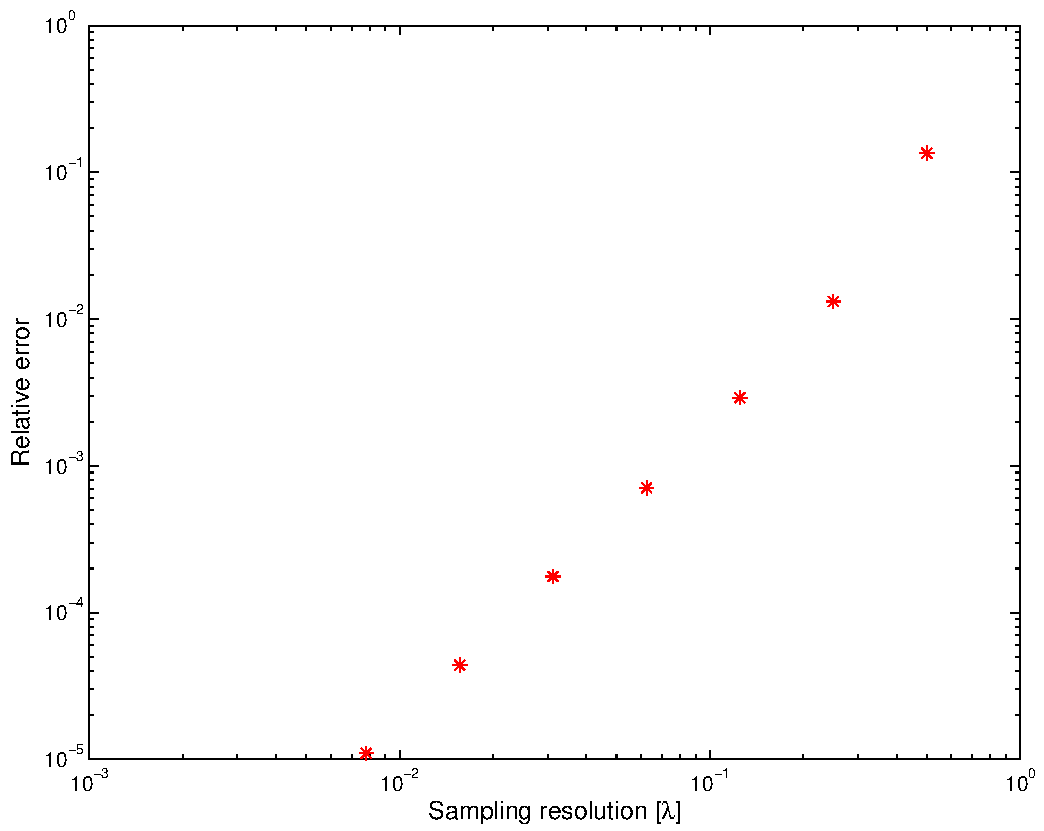
\includegraphics[width=12cm]{boxSamplingVect}
\caption{Relative error between N2F and direct far fields detectors for several sampling resolutions.}
\label{fig:boxSamplingVect}
\end{figure} 
